\documentclass[11pt]{article}
%% Packages:

\usepackage{amsmath}
\usepackage[document]{ragged2e}
\usepackage{titlesec}
\usepackage{float}
\usepackage{graphicx}
\usepackage{caption}
\usepackage{subcaption}
\usepackage[dvipsnames]{xcolor}
\usepackage[T1]{fontenc}
\usepackage{helvet}
\usepackage[hidelinks]{hyperref}
\usepackage[margin=2cm]{geometry}
\usepackage{amssymb}
\usepackage{enumitem}
\usepackage{comment}
\usepackage{soul}

%% Personalized adjustements: 

% Math operator:
\DeclareMathOperator{\sech}{sech}

% VUB colors: 
\definecolor{orange}{RGB}{234, 82, 0} 
\definecolor{blue}{RGB}{26, 55, 101}

% Margins:
\addtolength{\skip\footins}{0.3 cm}
\renewcommand*\footnoterule{}

% Adjustement of section, subsection & subsubsection: 

\titleformat{\section}[block]
{\normalfont\Large\bfseries \fontfamily{phv}\selectfont \color{orange}}
{\thesection}{0.5cm}{}

\titleformat{\subsection}[block]
{\normalfont\large\bfseries \fontfamily{phv}\selectfont \color{blue}}
{\thesubsection}{0.5cm}{}

\titleformat{\subsubsection}[block]
{\normalfont\small\bfseries \fontfamily{phv}\selectfont \color{blue}}
{\thesubsubsection}{0.5cm}{} % Assuming this contains necessary packages like amsmath, graphicx, subcaption, etc.
\usepackage{setspace}
\usepackage{graphicx}
\usepackage{subcaption}
\usepackage{parskip} % For paragraphs separated by vertical space instead of indent
\usepackage{indentfirst} % To indent the first paragraph of a section
\graphicspath{{Images/}}
%\setlength{\parindent}{1.5em} % User had this commented out, will respect that for now.
\usepackage{float} % For [H] option
\onehalfspacing

% Custom command for question environment if desired for formatting
\newenvironment{projectquestion}[1]
{\par\ थोड़ाvspace{\topsep}\noindent\textbf{#1}\ थोड़ा\quad\ignorespaces}
{\par\ थोड़ाvspace{\topsep}}

\begin{document}
	\justifying % Assuming this is a custom command for justification
	
	\begin{titlepage}
	\begin{center}
            \begin{figure}
                \centering
                
\includegraphics[scale=0.3]{Images/logo.png}
            \end{figure}
		\vspace*{\fill}
            \normalsize
            {\fontfamily{phv}\selectfont
            \textcolor{blue}{\textbf{ELEC-H401}}}\\
            \vspace{0.2cm}
		\Huge
            {\fontfamily{phv}\selectfont
            \textcolor{orange}{Design and Simulation of a DVB-C Transmission Chain}}\\
        \end{center}
	\begin{center}	
		\vspace{0.5cm}
            \Large
            {\fontfamily{phv}\selectfont
			\textcolor{blue}{\textbf{Hadislam Satouev\\
                                 	 Cédric Sipakam
             }}}\\
	\end{center}
        \vspace*{\fill}
        \begin{FlushRight}
            {\fontfamily{phv}\selectfont
            \textcolor{orange}{Professor}}\\
            {\fontfamily{phv}\selectfont
            \textcolor{blue}{François Horlin}}\\
            \vspace{0.6cm}
            {\fontfamily{phv}\selectfont
            \textcolor{orange}{Teaching Assistants}}\\
            {\fontfamily{phv}\selectfont
            \textcolor{blue}{
                ....\\
                 ....
            }}\\
            \vspace{0.6cm}
            {\fontfamily{phv}\selectfont
            \textcolor{orange}{Academic Year}}\\
            {\fontfamily{phv}\selectfont
            \textcolor{blue}{2024 - 2025}}\\
            \vspace{0.6cm}
            {\fontfamily{phv}\selectfont
            \textcolor{orange}{Faculty}}\\
            {\fontfamily{phv}\selectfont
            \textcolor{blue}{Electrical Engineering}}
        \end{FlushRight}



\end{titlepage} % Assuming this is your title page
	\tableofcontents
	\newpage
	\listoffigures
	
	\newpage
	\section*{Introduction}{\addcontentsline{toc}{section}{Introduction}}
	This project focuses on designing and simulating a Digital Video Broadcasting Cable transmission chain using Matlab.
	The main goal is to model and analyze the components of a typical modem. The first part of this project includes establishing an optimal communication chain over an ideal Additive White Gaussian Noise channel, mapping the signal into symbols, Nyquist filtering, and evaluating the performance of the system through Bit Error Rate simulations for Quadrature Amplitude Modulation signals. The second part revolves around the design and assessment of time and frequency synchronization algorithms. This encompasses evaluating the impact of synchronization errors such as carrier phase and frequency offset and sample time shift. The algorithms used for this purpose are the Gardner Algorithm for time recovery, and a differential cross-correlator for joint frame and frequency acquisition. Afterwards, their effectiveness is demonstrated \textcolor{red}{through convergence analysis and residual error evaluation (double check)}. \textcolor{red}{The study also explores phase interpolation techniques to mitigate remaining phase drifts. Finally, the project aims to validate the simulated chain through real-life experimentation on a Hybrid Fiber-Coax setup using Adalm-Pluto hardware, and to compare the simulated performance with experimental observations.}
	
	
	\section{Optimal Communication Chain over the Ideal Channel}
	Figure \ref{fig:com-chain} shows the simulated DVB-C baseband communication chain. The transmitter generates bits, maps them to QAM symbols, upsamples, and shapes them with a half-root Nyquist filter. The receiver uses a matched filter, downsamples, and demapps symbols. LDPC coding is not implemented.
	
	\begin{figure}[H]
		\centering
		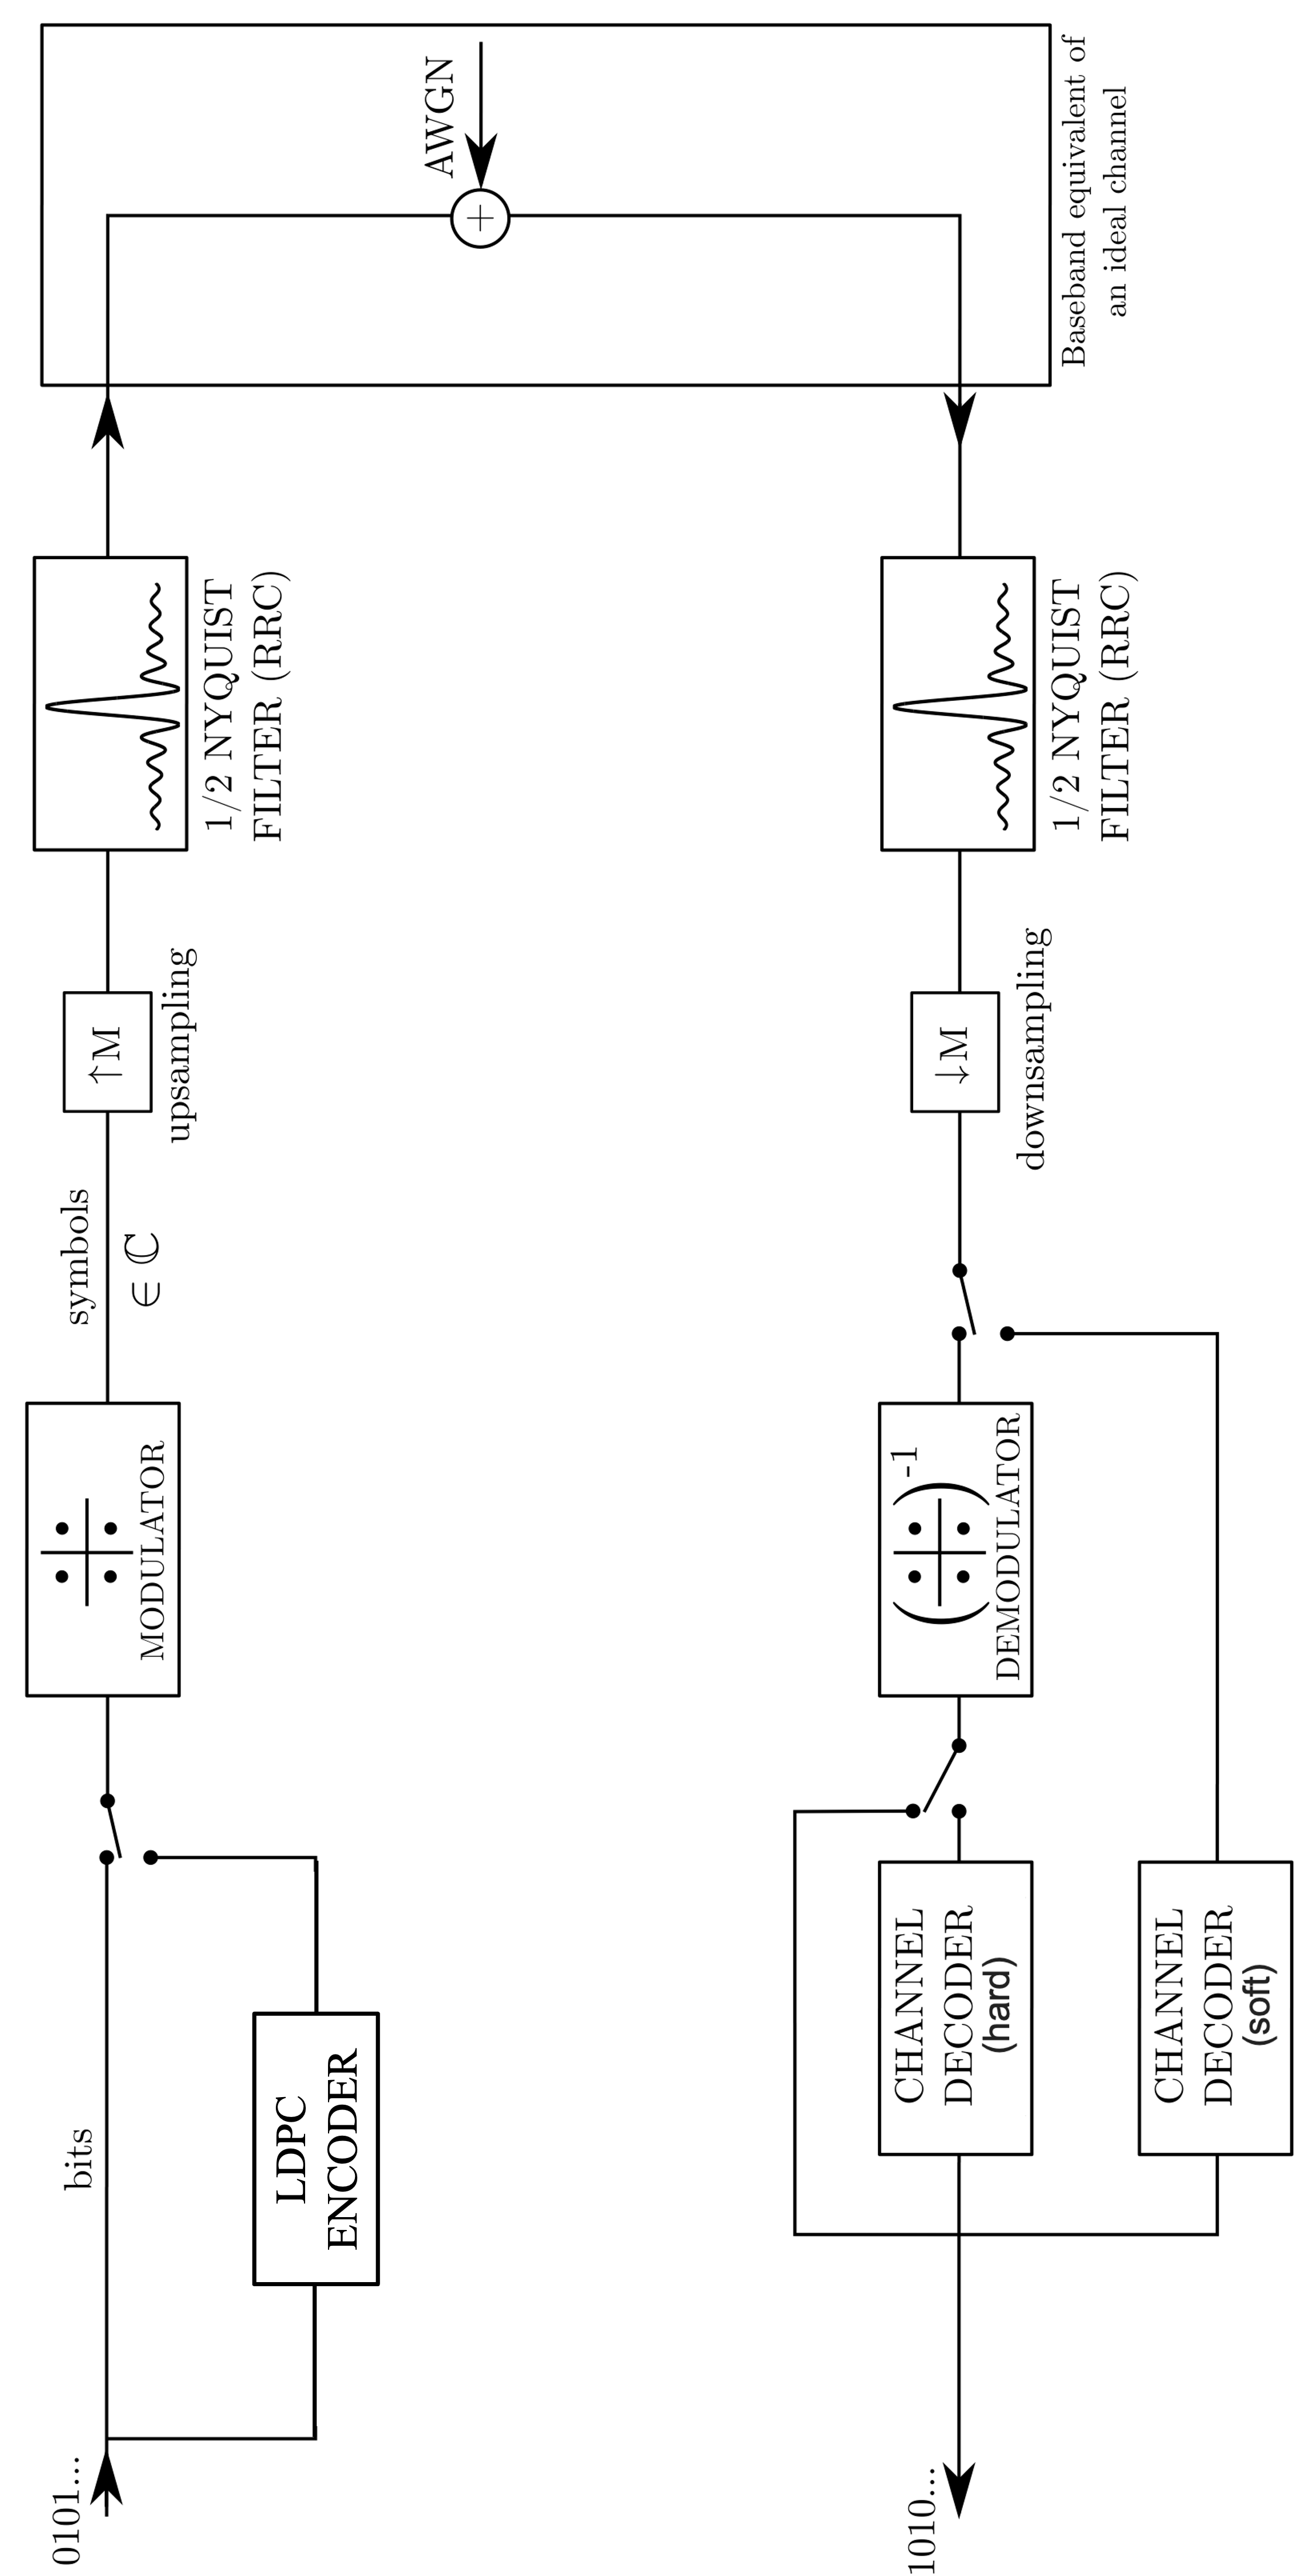
\includegraphics[angle=-90, width=0.7\linewidth]{Images/com-chain}
		\caption{Block diagram of the communication system.}
		\label{fig:com-chain}
	\end{figure}
	
	Symbol mapping transforms random bits into complex symbols. Demapping uses Maximum Likelihood (ML) to select the constellation symbol $\underline{s}_{m}$ minimizing Euclidean distance to the received sample $\underline{r}$:
	\begin{equation}
		\tilde{\underline{s}}_{m}^{ML} = \arg\min_{\underline{s}_{m}} \left(\sum_{k=1}^{K}(r_{k}-s_{mk})^{2}\right)
	\end{equation}
	This is equivalent to maximizing $\ln p(\underline{r}|\underline{s}_{m})$ for an AWGN channel.
	
	Nyquist filtering uses a root-raised cosine (RRC) filter $g(t)$ for pulse shaping and its matched version $g^*(-t)$ at the receiver. Their convolution $h(t) = g(t) \otimes g^*(-t)$ satisfies the Nyquist zero ISI criterion at $T_{symb}$ intervals: $h(kT_{symb}) = \delta[k]$. The RRC frequency response $G(f) = \sqrt{H(f)}$, where $H(f)$ is the RC filter response:
	\begin{equation}
		H(f) = \begin{cases}
			T_{symb} & 0 \le |f| < \frac{1-\beta}{2T_{symb}} \\      
			\frac{T_{symb}}{2} \left(1 + \cos\left[\frac{\pi T_{symb}}{\beta}\left(|f| - \frac{1-\beta}{2T_{symb}}\right)\right]\right) & \frac{1-\beta}{2T_{symb}} \le |f| \le \frac{1+\beta}{2T_{symb}} \\      
			0 & |f| > \frac{1+\beta}{2T_{symb}}
		\end{cases}
	\end{equation}
	Figure \ref{fig:nyquist-filter-combined} shows the simulated $H(f)$ for $R_{symb} = 5 \text{ Msymb/s}$ and $\beta = 0.2$, confining the signal to a 6 MHz bandwidth, and $h(t)$ illustrating ISI cancellation at $kT_{symb}$.
	
	\begin{figure}[H]
		\centering
		\begin{subfigure}[b]{0.48\textwidth}
			\centering
			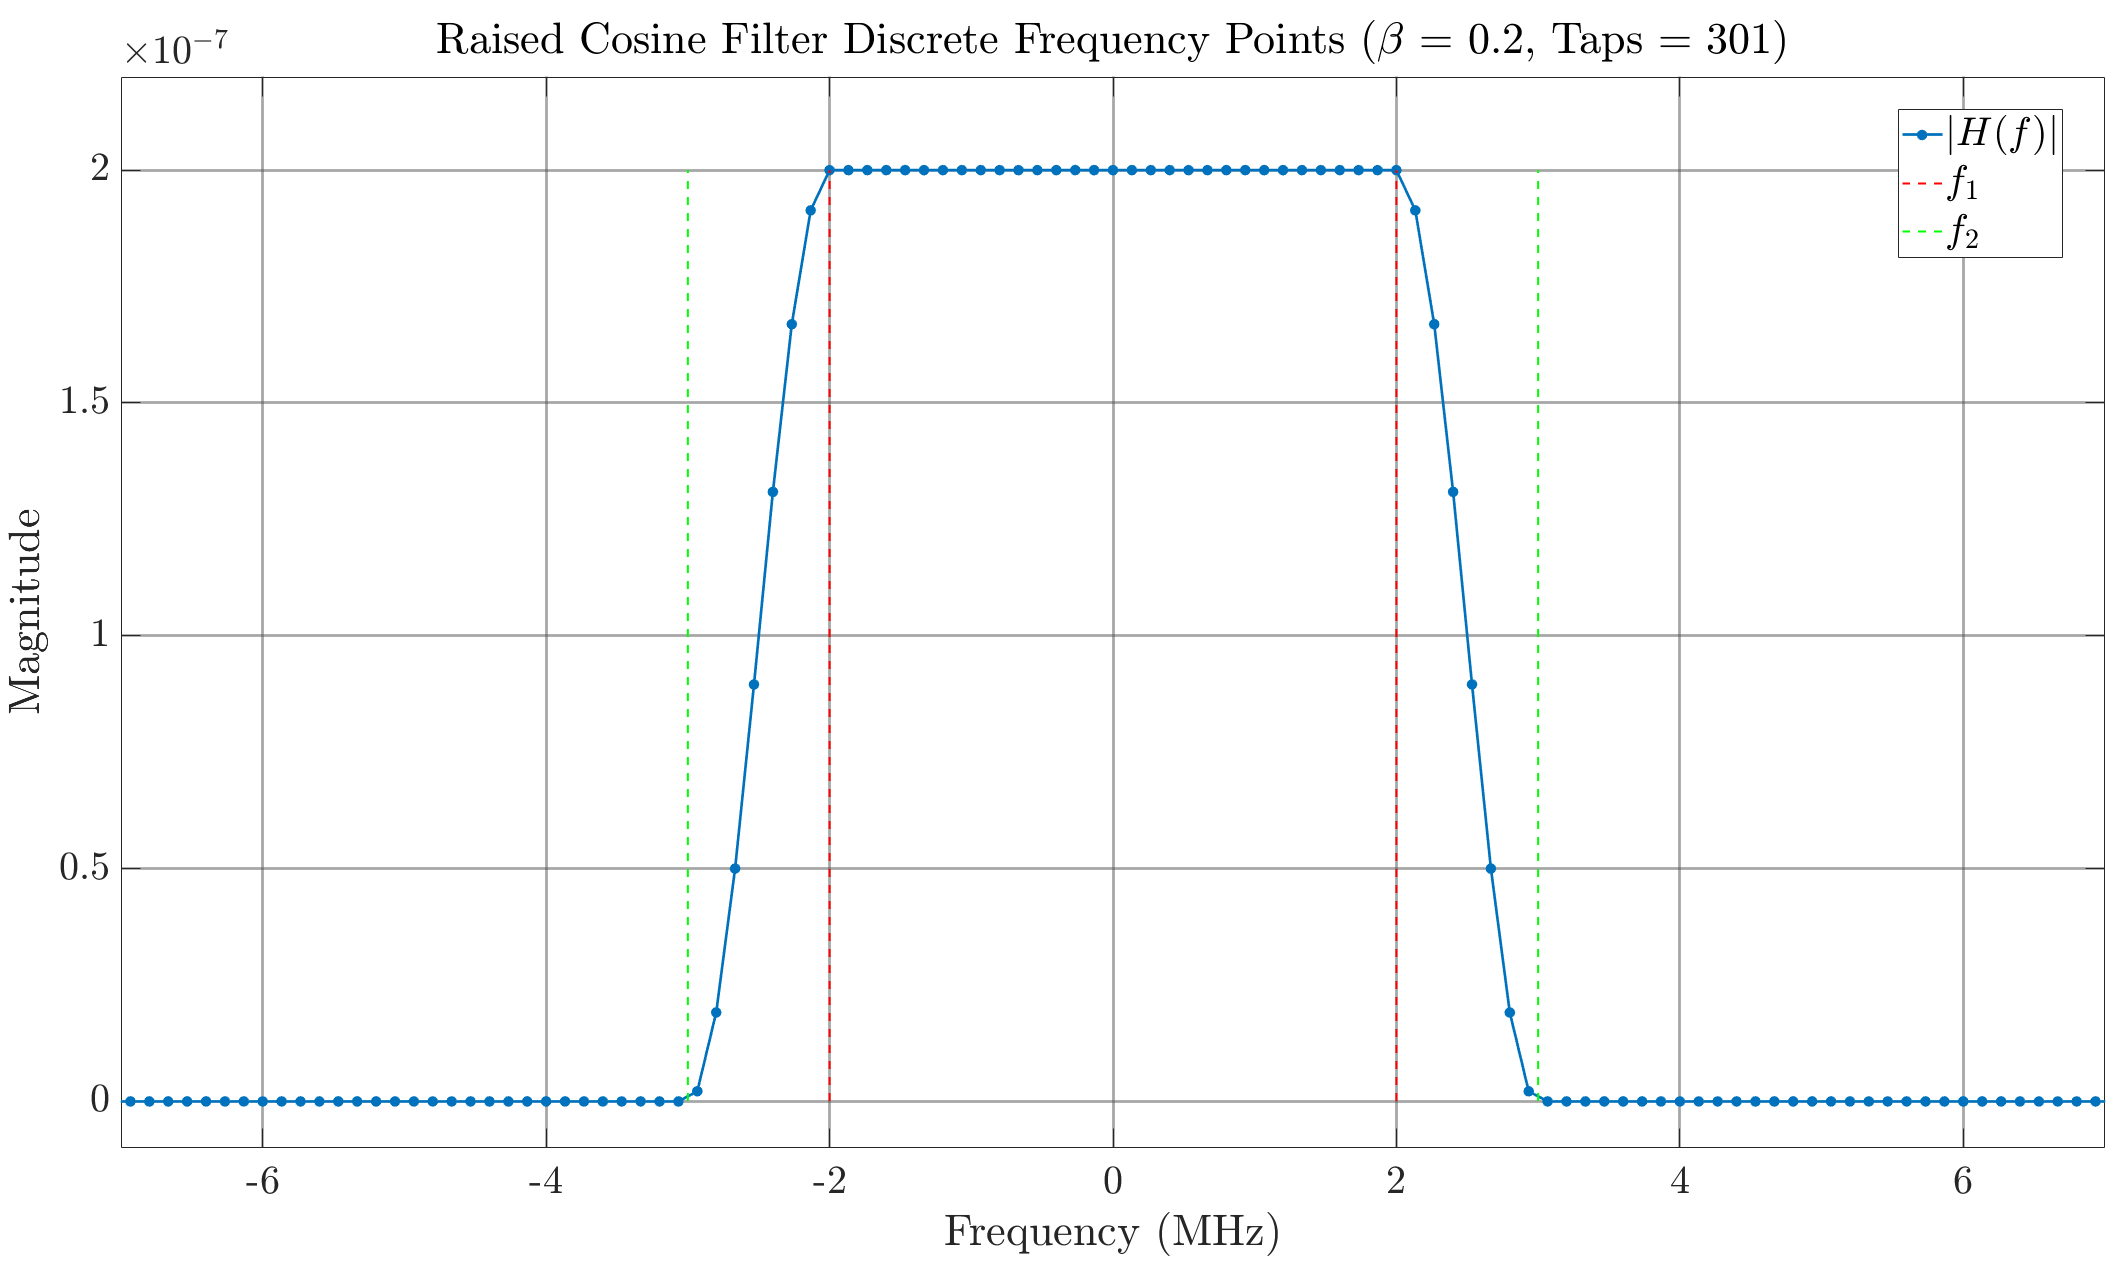
\includegraphics[width=\linewidth]{Images/h-rc-freq}
			\caption{RC Filter Frequency Response ($\beta = 0.2$).}
			\label{fig:h-rc-freq_compact}
		\end{subfigure}
		\hfill
		\begin{subfigure}[b]{0.48\textwidth}
			\centering
			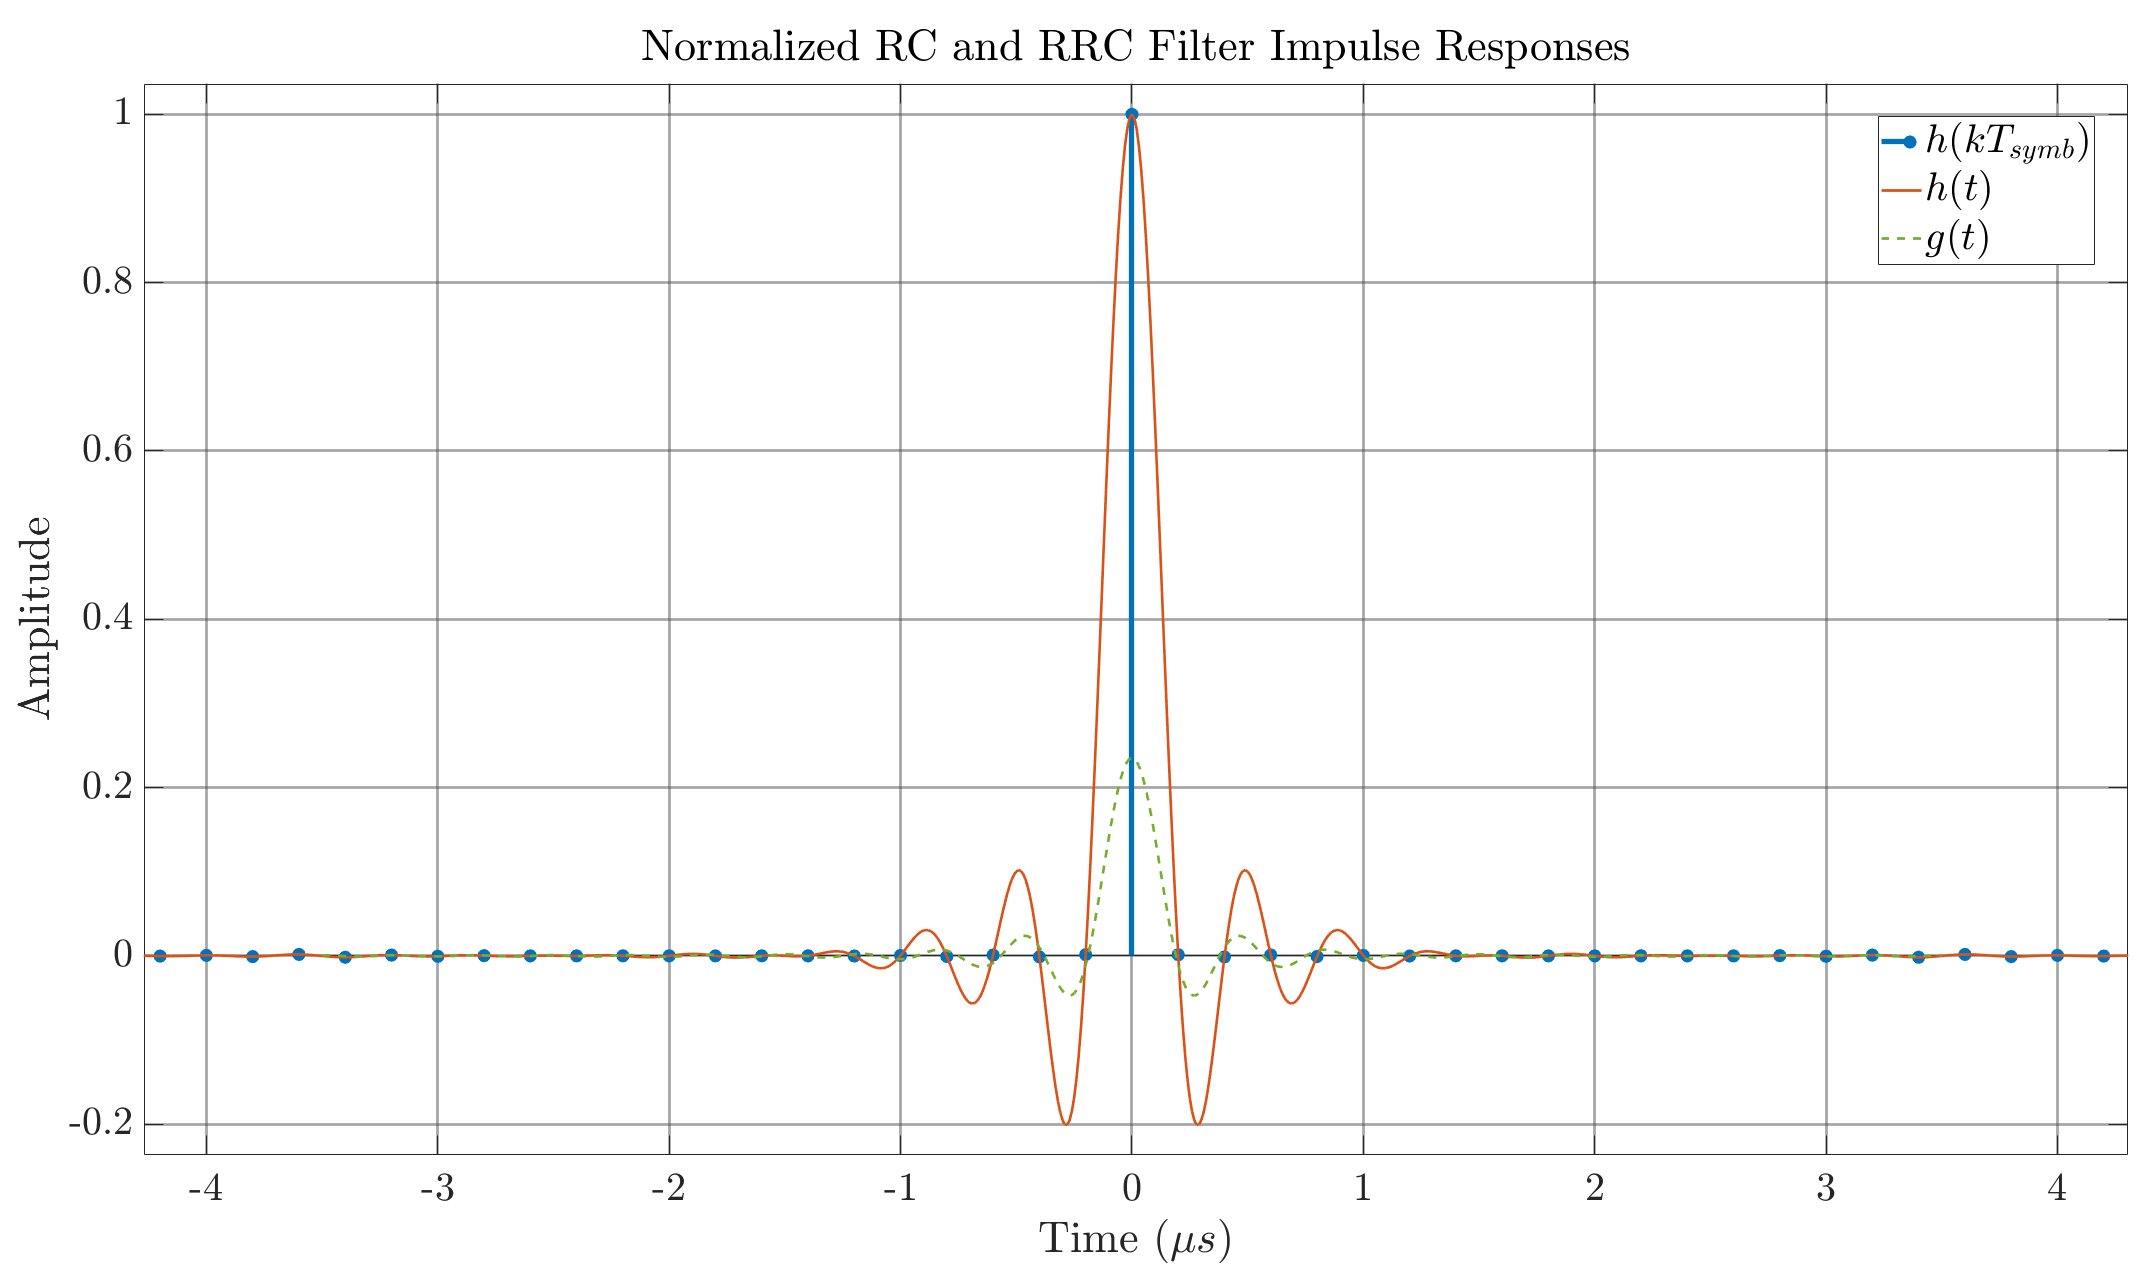
\includegraphics[width=\linewidth]{Images/h-rc}
			\caption{Normalized RC and RRC Impulse Responses.}
			\label{fig:h-rc_compact}
		\end{subfigure}
		\caption{Simulated Nyquist filter characteristics.}
		\label{fig:nyquist-filter-combined}
	\end{figure}
	
	AWGN $n(t)$ is added to the signal $s(t)$, so $r(t) = s(t) + n(t)$. After matched filtering and sampling, $y[k] = I[k] + n_o[k]$, where $n_o[k]$ is complex Gaussian noise with variance $N_0/2$ per component. Performance is measured by BER vs. $E_b/N_0$. The theoretical $P_b$ for M-QAM is:
	\begin{equation}
		P_b \approx \frac{4}{\log_2 M} \left(1 - \frac{1}{\sqrt{M}}\right) Q\left(\sqrt{\frac{3 (\log_2 M)^2}{M-1} \frac{E_b}{N_0}}\right)
	\end{equation}
	Figure \ref{fig:ber-mod_cont} validates theoretical BER curves. Higher-order QAMs achieve higher data rates but require more power. Figure \ref{fig:constellations-noise_cont} shows the effect of AWGN on 16-QAM symbols before and after matched filtering, the latter showing tighter clusters due to SNR maximization.
	
	\begin{figure}[H]
		\centering
		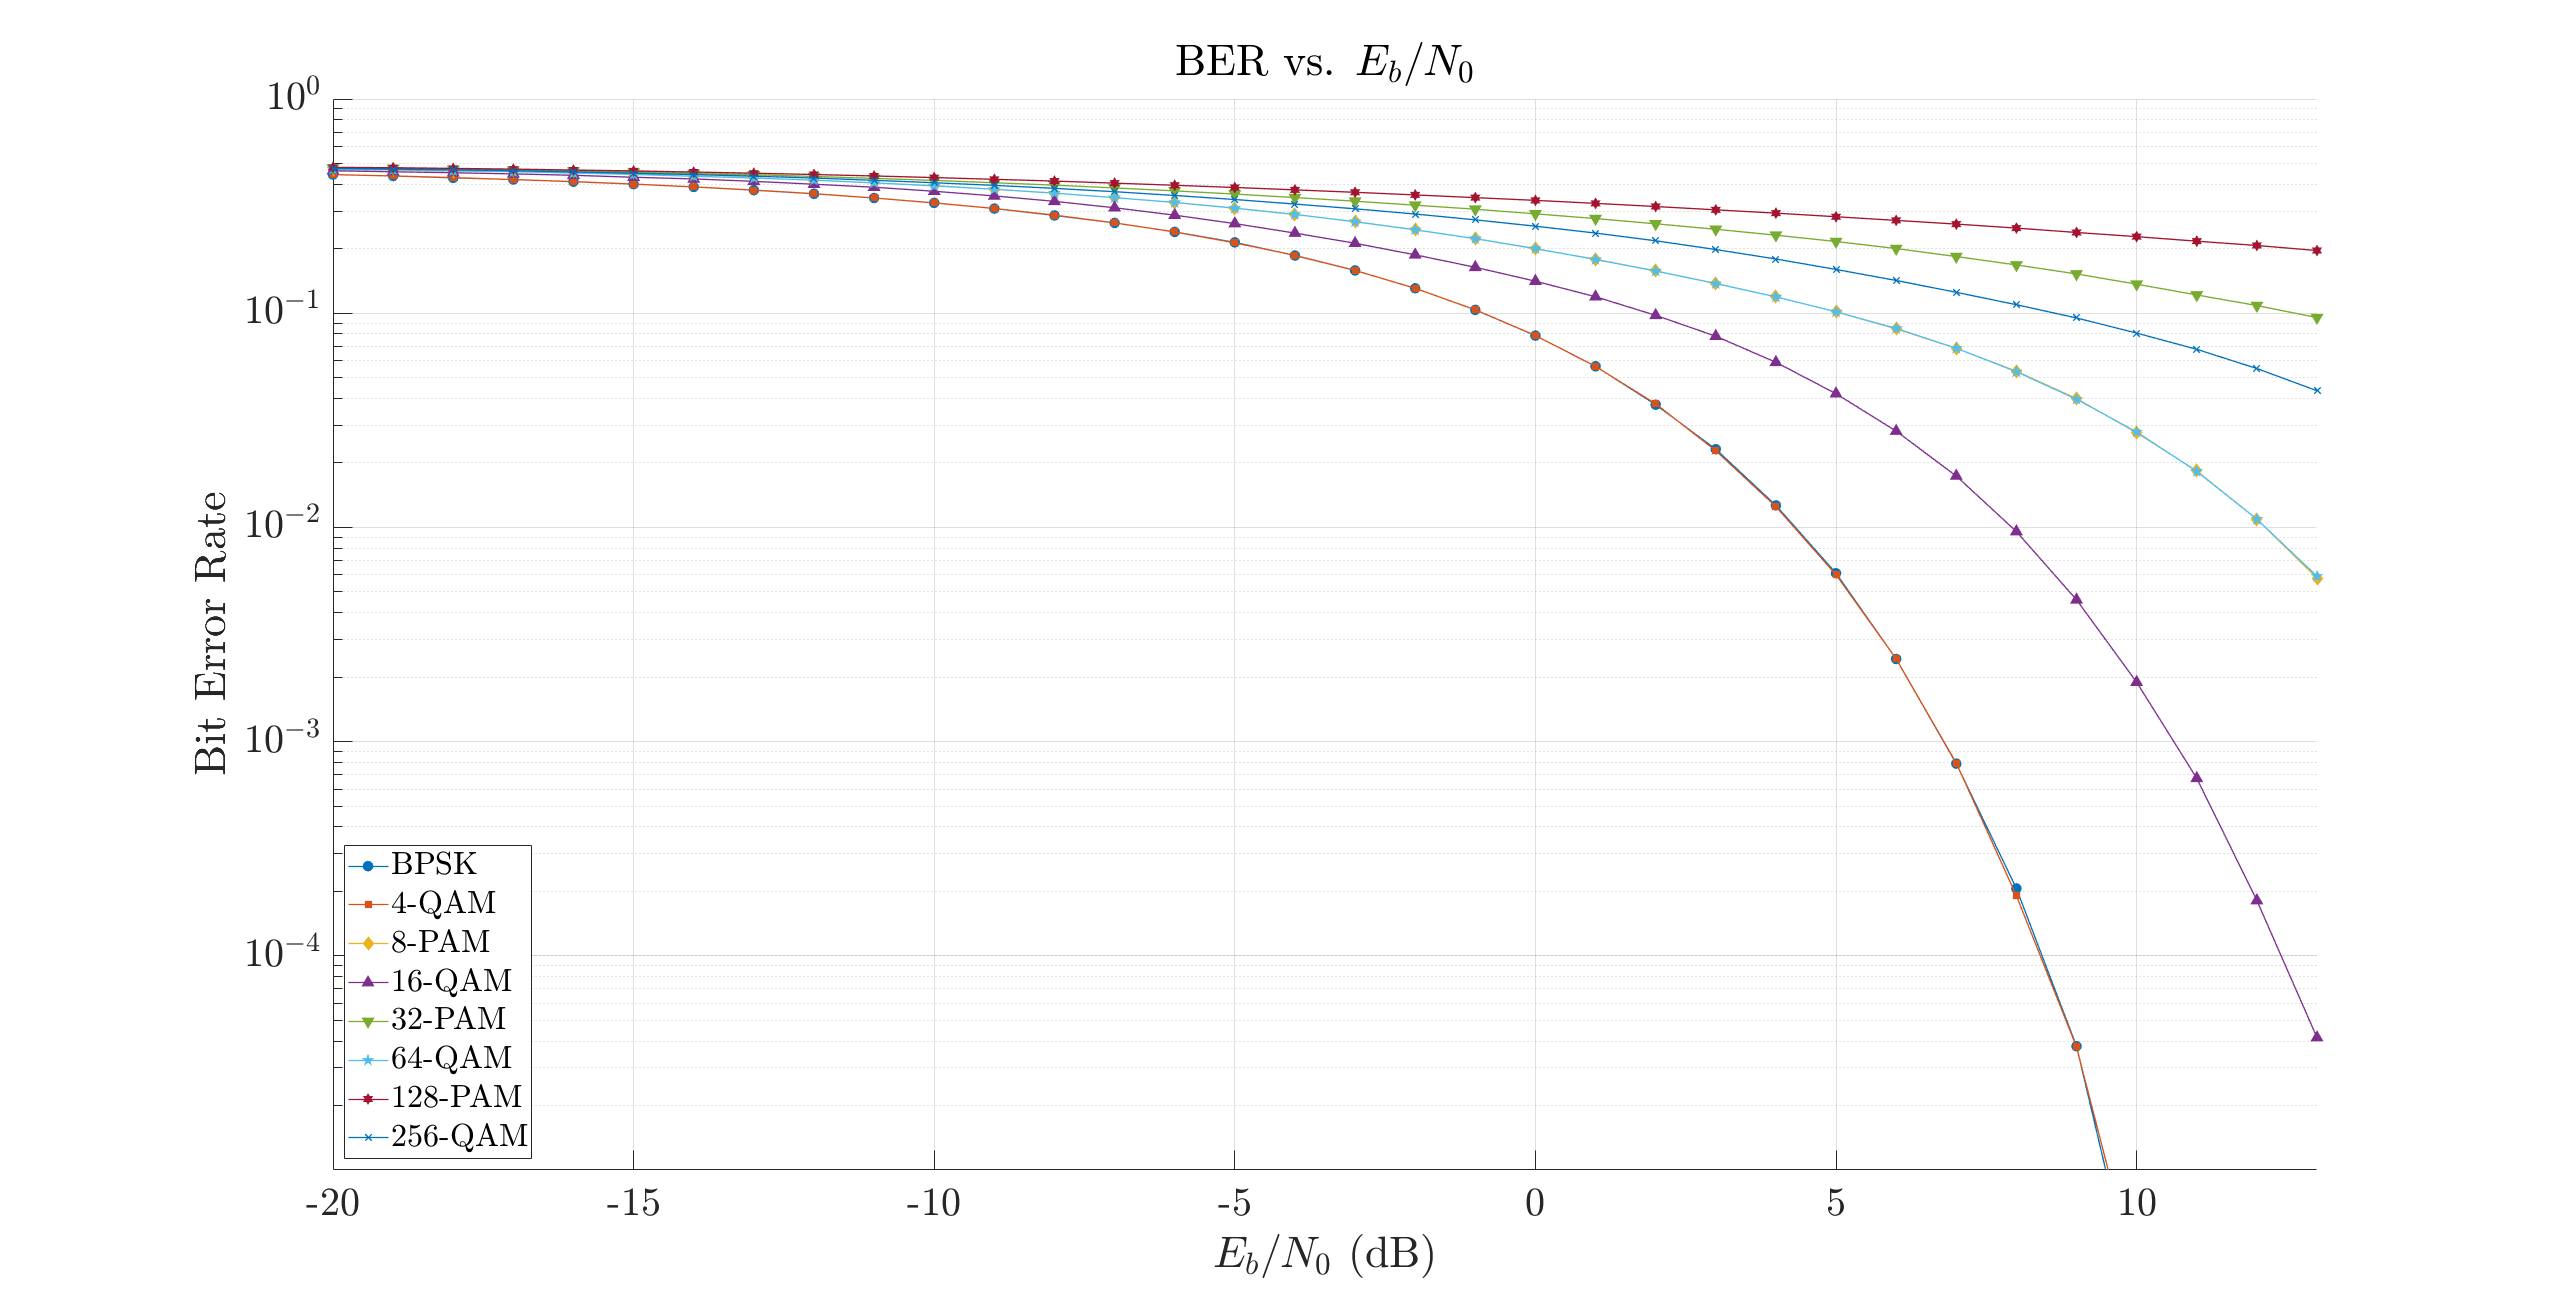
\includegraphics[width=0.7\linewidth]{Images/ber-mod.png}
		\caption{Simulated BER vs. $E_b/N_0$ for various modulation types.}
		\label{fig:ber-mod_cont}
	\end{figure}
	
	\begin{figure}[H]
		\centering
		\begin{subfigure}{0.48\textwidth}
			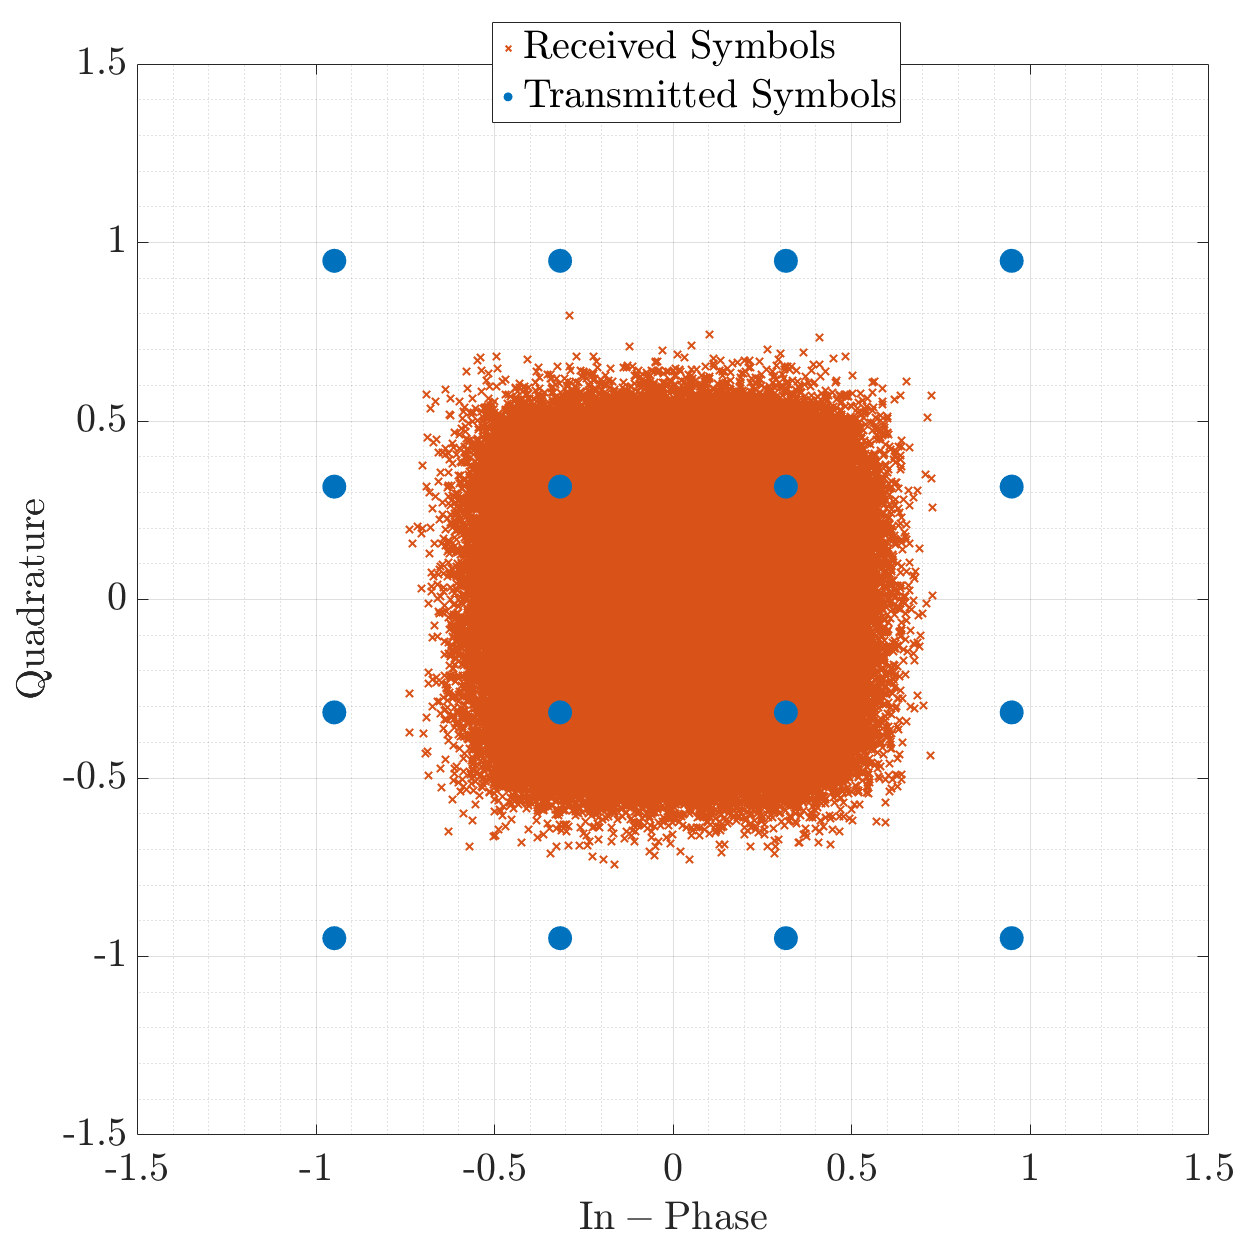
\includegraphics[width=\linewidth]{Images/const-noisy.png}
			\caption{Noisy 16-QAM before matched filter.}
			\label{fig:const-noisy_cont_compact}
		\end{subfigure}\hfill
		\begin{subfigure}{0.48\textwidth}
			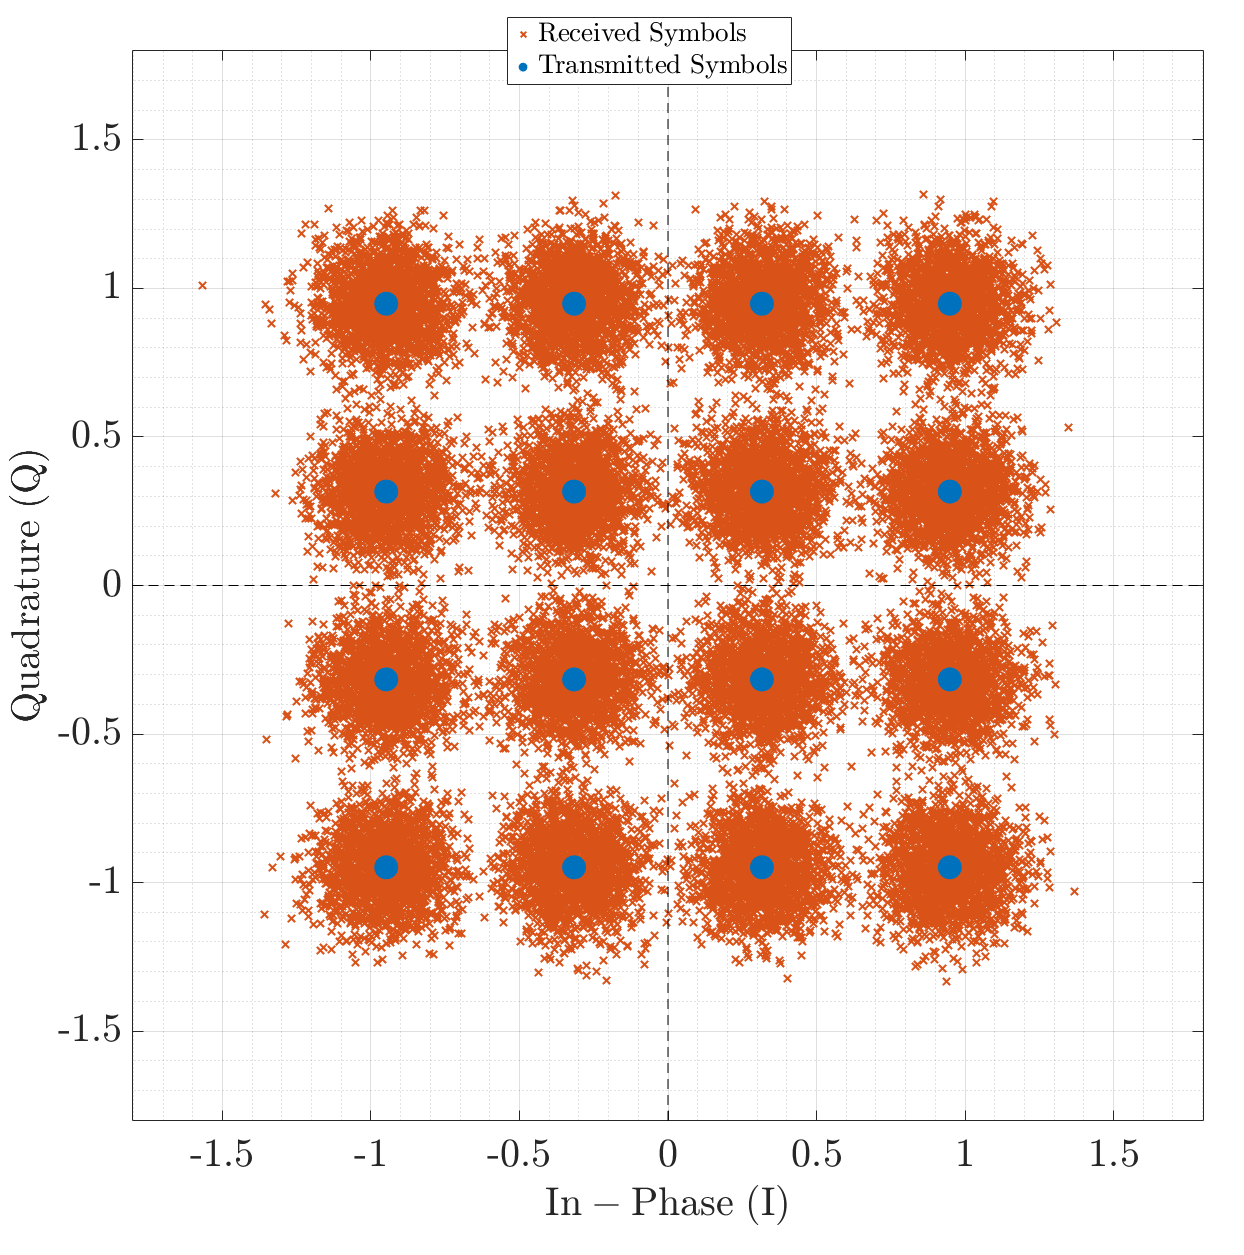
\includegraphics[width=\linewidth]{Images/const-filtered-down.png}      
			\caption{16-QAM after matched filtering.}
			\label{fig:const-filtered-down_cont_compact}
		\end{subfigure}
		\caption{Effect of AWGN and matched filtering on 16-QAM ($\frac{E_b}{N_0} = 15$ dB).}
		\label{fig:constellations-noise_cont}
	\end{figure}
	
	\subsection*{Questions: Optimal Communication Chain}
	\begin{projectquestion}{Baseband vs. Bandpass Implementation:}
		Working with baseband equivalent models reduces complexity by avoiding high carrier frequencies, allowing lower simulation sampling rates and modular design of modulation/demodulation stages.
	\end{projectquestion}
	
	\begin{projectquestion}{Sample Rate Selection:}
		The Matlab sampling rate $F_s$ must be at least twice the maximum signal frequency $F_{max}$ (Nyquist criterion) to prevent aliasing. For an RRC filter with roll-off $\beta$, $F_{max} = (1+\beta)/(2T_{symb})$. Thus, the oversampling factor $M$ must ensure $F_s = M/T_{symb} \ge 2 F_{max}$.
	\end{projectquestion}
	
	\begin{projectquestion}{Simulating $E_b/N_0$ Ratio:}
		Noise power $P_n = N_0 F_s$. $N_0$ is derived from the target $E_b/N_0$ and calculated bit energy $E_b$. $E_b = E_s / \log_2(M)$, where $E_s$ is average symbol energy. Complex noise $n(t) = \sqrt{P_n/2}(X+jY)$ is generated with $X, Y \sim \mathcal{N}(0,1)$.
	\end{projectquestion}
	
	\begin{projectquestion}{Number and Length of Data Packets:}
		The number of bits per packet must be a multiple of $\log_2(M)$ for M-QAM to avoid unused bits. Total transmitted bits must be sufficient for statistically relevant BER estimation, typically such that at least 10-100 errors are observed for the target BER.
		\end{projectquestion>
			
			\begin{projectquestion}{Supported Bit Rate vs. Physical Bandwidth:}
				The two-sided Nyquist bandwidth is $B = (1+\beta)/T_{symb}$. The bit rate $R_b = (\log_2 M) / T_{symb} = (\log_2 M) \cdot R_{symb}$. Thus $R_b = R_{symb} \cdot \log_2 M = \frac{B}{1+\beta} \log_2 M$.
			\end{projectquestion}
			
			\begin{projectquestion}{Trade-off: Capacity vs. Reliability (Constellation Size):}
				Larger constellations (higher M) increase capacity (more bits/symbol, higher $R_b$ for fixed bandwidth). However, constellation points are closer, reducing Euclidean distance and increasing susceptibility to noise, thus degrading BER for a given $E_b/N_0$ (lower reliability).
			\end{projectquestion}
			
			\begin{projectquestion}{Choice of Half-Root Nyquist Filter:}
				RRC filters are used because: 1) When paired (transmitter and matched receiver filter), they form an overall Nyquist filter, ensuring zero ISI at correct sampling instants. 2) The matched filter maximizes SNR at the detector input. 3) They provide good spectral containment.
			\end{projectquestion}
			
			\begin{projectquestion}{Optimal Demodulator Implementation:}
				The optimal demodulator for AWGN channels uses a filter matched to the transmitted pulse shape $g(t)$, i.e., $g^*(-t)$, followed by sampling at symbol instants $kT_{symb}$. This maximizes the output SNR.
			\end{projectquestion}
			
			\begin{projectquestion}{Optimal Detector Implementation:}
				The optimal detector minimizes symbol error probability. For equiprobable symbols in AWGN, this corresponds to the Maximum Likelihood (ML) criterion: choose symbol $s_m$ that maximizes $p(r|s_m)$. This simplifies to minimizing the Euclidean distance: $\hat{s}_{ML} = \arg\min_{s_m} ||r - s_m||^2$.
			\end{projectquestion}
			
			\section{Time and Frequency Synchronization}
			Synchronization aligns receiver timing and carrier with the transmitter. Errors include Carrier Frequency Offset ($\Delta f$), Phase Offset ($\phi_0$), and Sample Time Shift ($t_0$), illustrated in Figure \ref{fig:sync-errors-conceptual}.
			
			\begin{figure}[H]
				\centering
				\begin{subfigure}[b]{0.45\textwidth} % Adjusted width
					\centering
					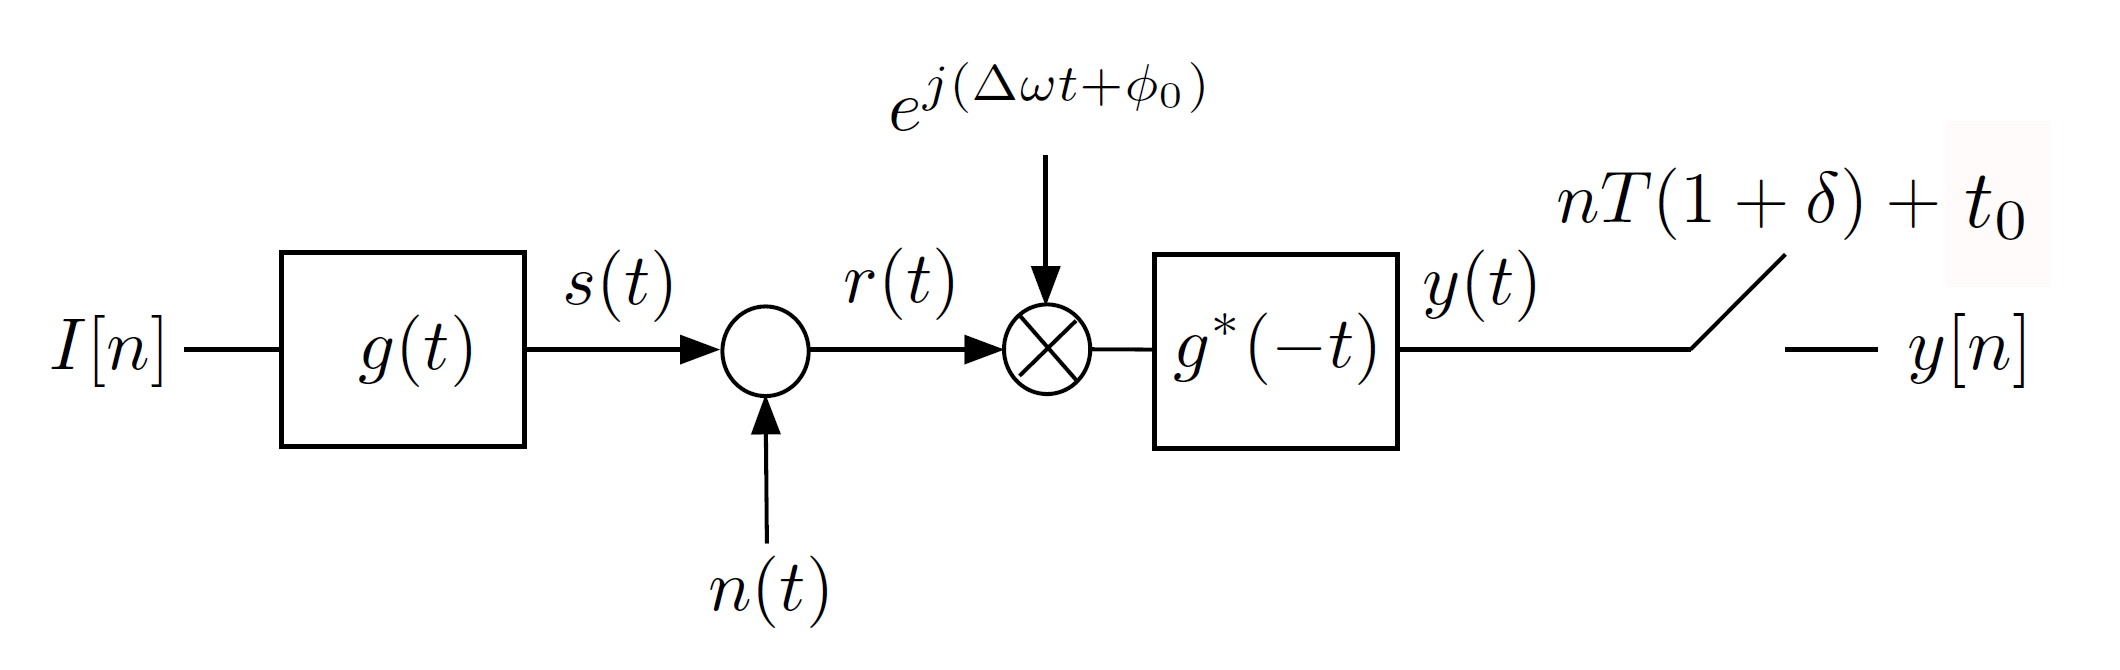
\includegraphics[width=\linewidth]{Images/sync-errors-conceptual} 
					\caption{Synchronization mismatches.}
					\label{fig:sync-errors-conceptual_compact}
				\end{subfigure}
				\hfill
				\begin{subfigure}[b]{0.45\textwidth} % Adjusted width
					\centering
					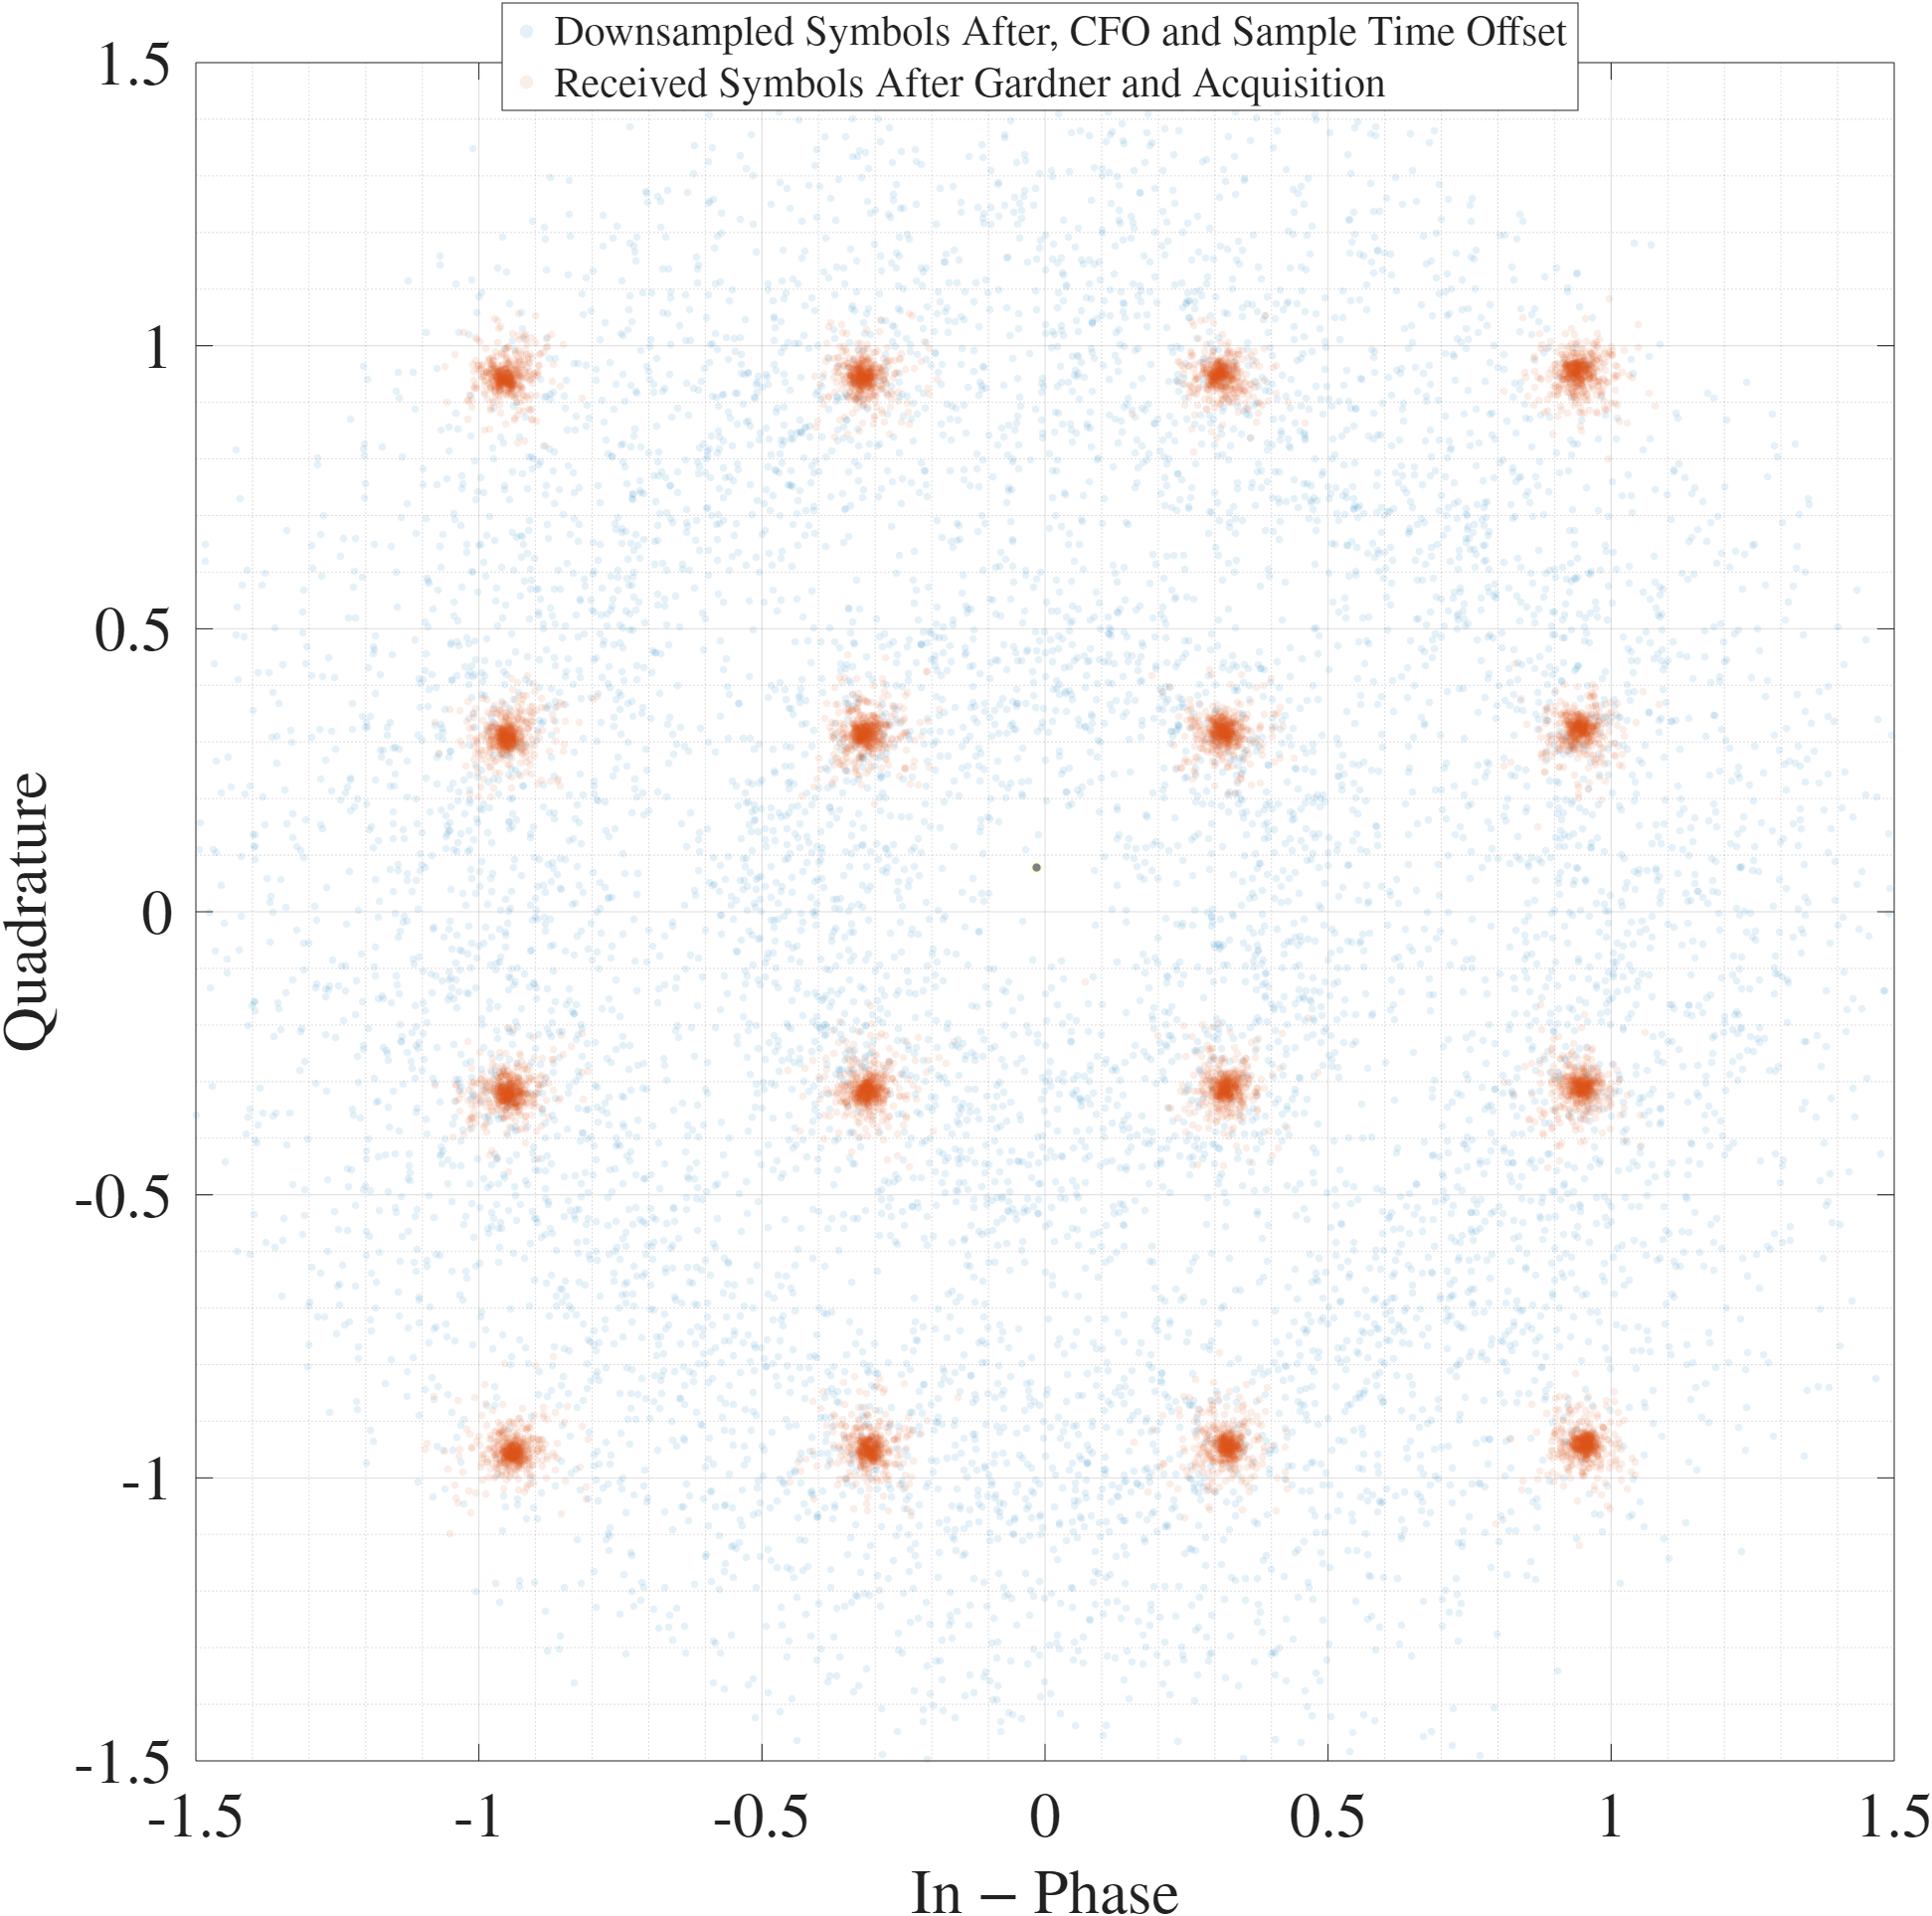
\includegraphics[width=\linewidth]{Images/const-corrected.png} 
					\caption{16-QAM: initial errors (blue) vs. post-sync (red).}
					\label{fig:const-corrected_compact}
				\end{subfigure}
				\caption{Synchronization challenges and overall correction impact ($E_b/N_0 = 20$ dB for (b)).}
				\label{fig:sync_overview_and_result}
			\end{figure}
			
			Synchronization errors degrade performance. $\phi_0$ rotates the constellation ($y[n] = I[n]e^{j\phi_0}$). $\Delta f$ causes phase drift ($y[n] = I[n]e^{j(2\pi \Delta f nT_{symb} + \phi_0')}$) and ISI due to filter mismatch. $t_0$ causes attenuation and ISI: $y[n] = I[n]h(t_0) + \sum_{m \neq n} I[m]h((n-m)T_{symb} + t_0)$. Figures \ref{fig:ber_sync_errors} and \ref{fig:const_sync_errors} show these impacts on BER and 16-QAM constellations.
			
			\begin{figure}[H]
				\centering
				\begin{subfigure}[b]{0.48\textwidth}
					\centering
					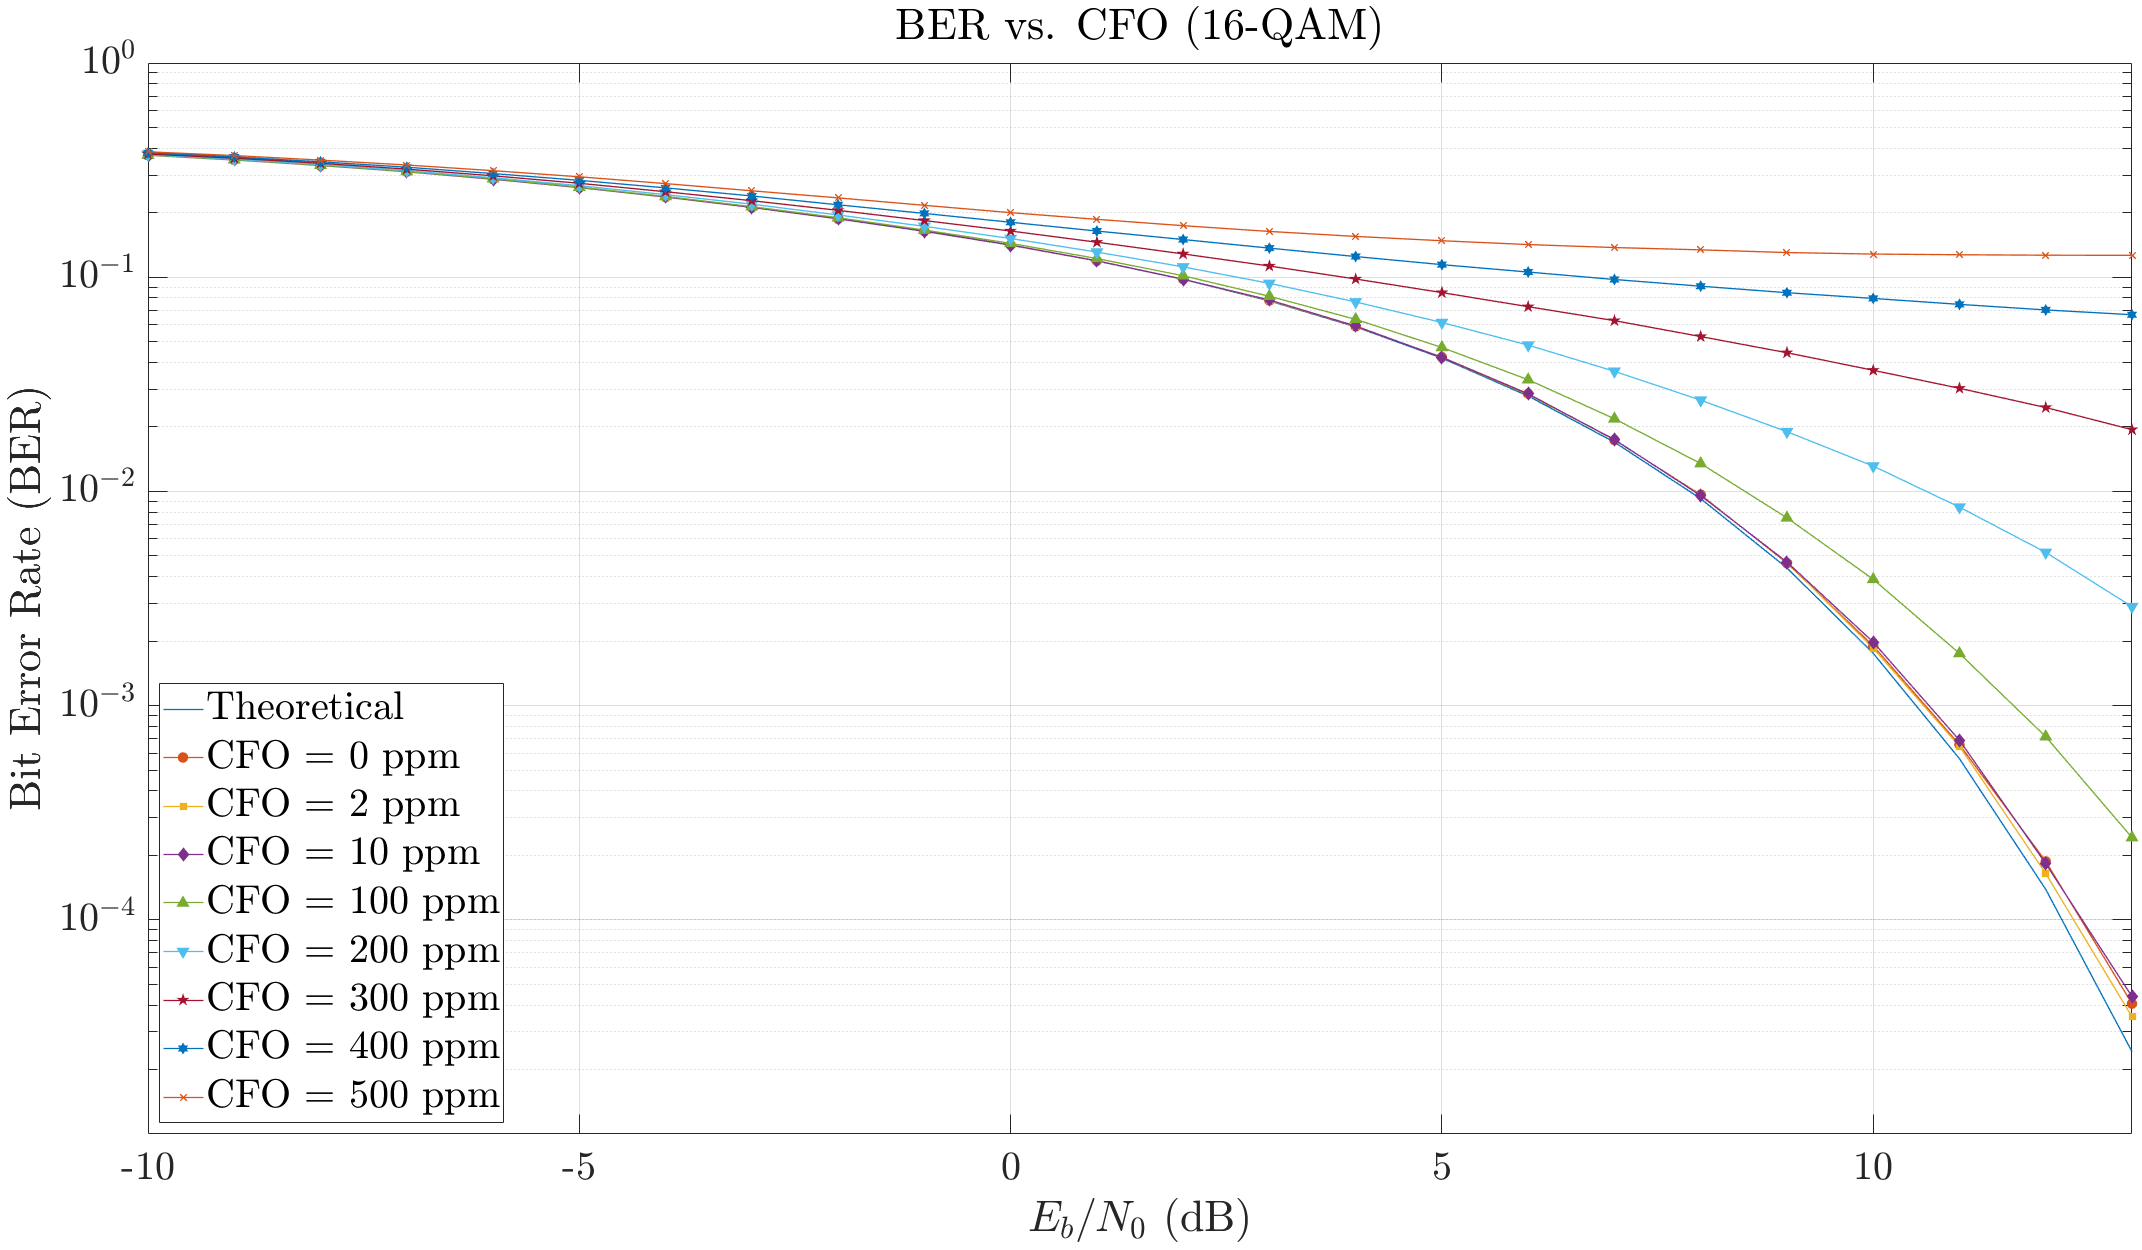
\includegraphics[width=\linewidth]{Images/ber-cfo}
					\caption{BER vs. $E_b/N_0$ for varying CFO.}
					\label{fig:ber-cfo_compact}
				\end{subfigure}
				\hfill
				\begin{subfigure}[b]{0.48\textwidth}
					\centering
					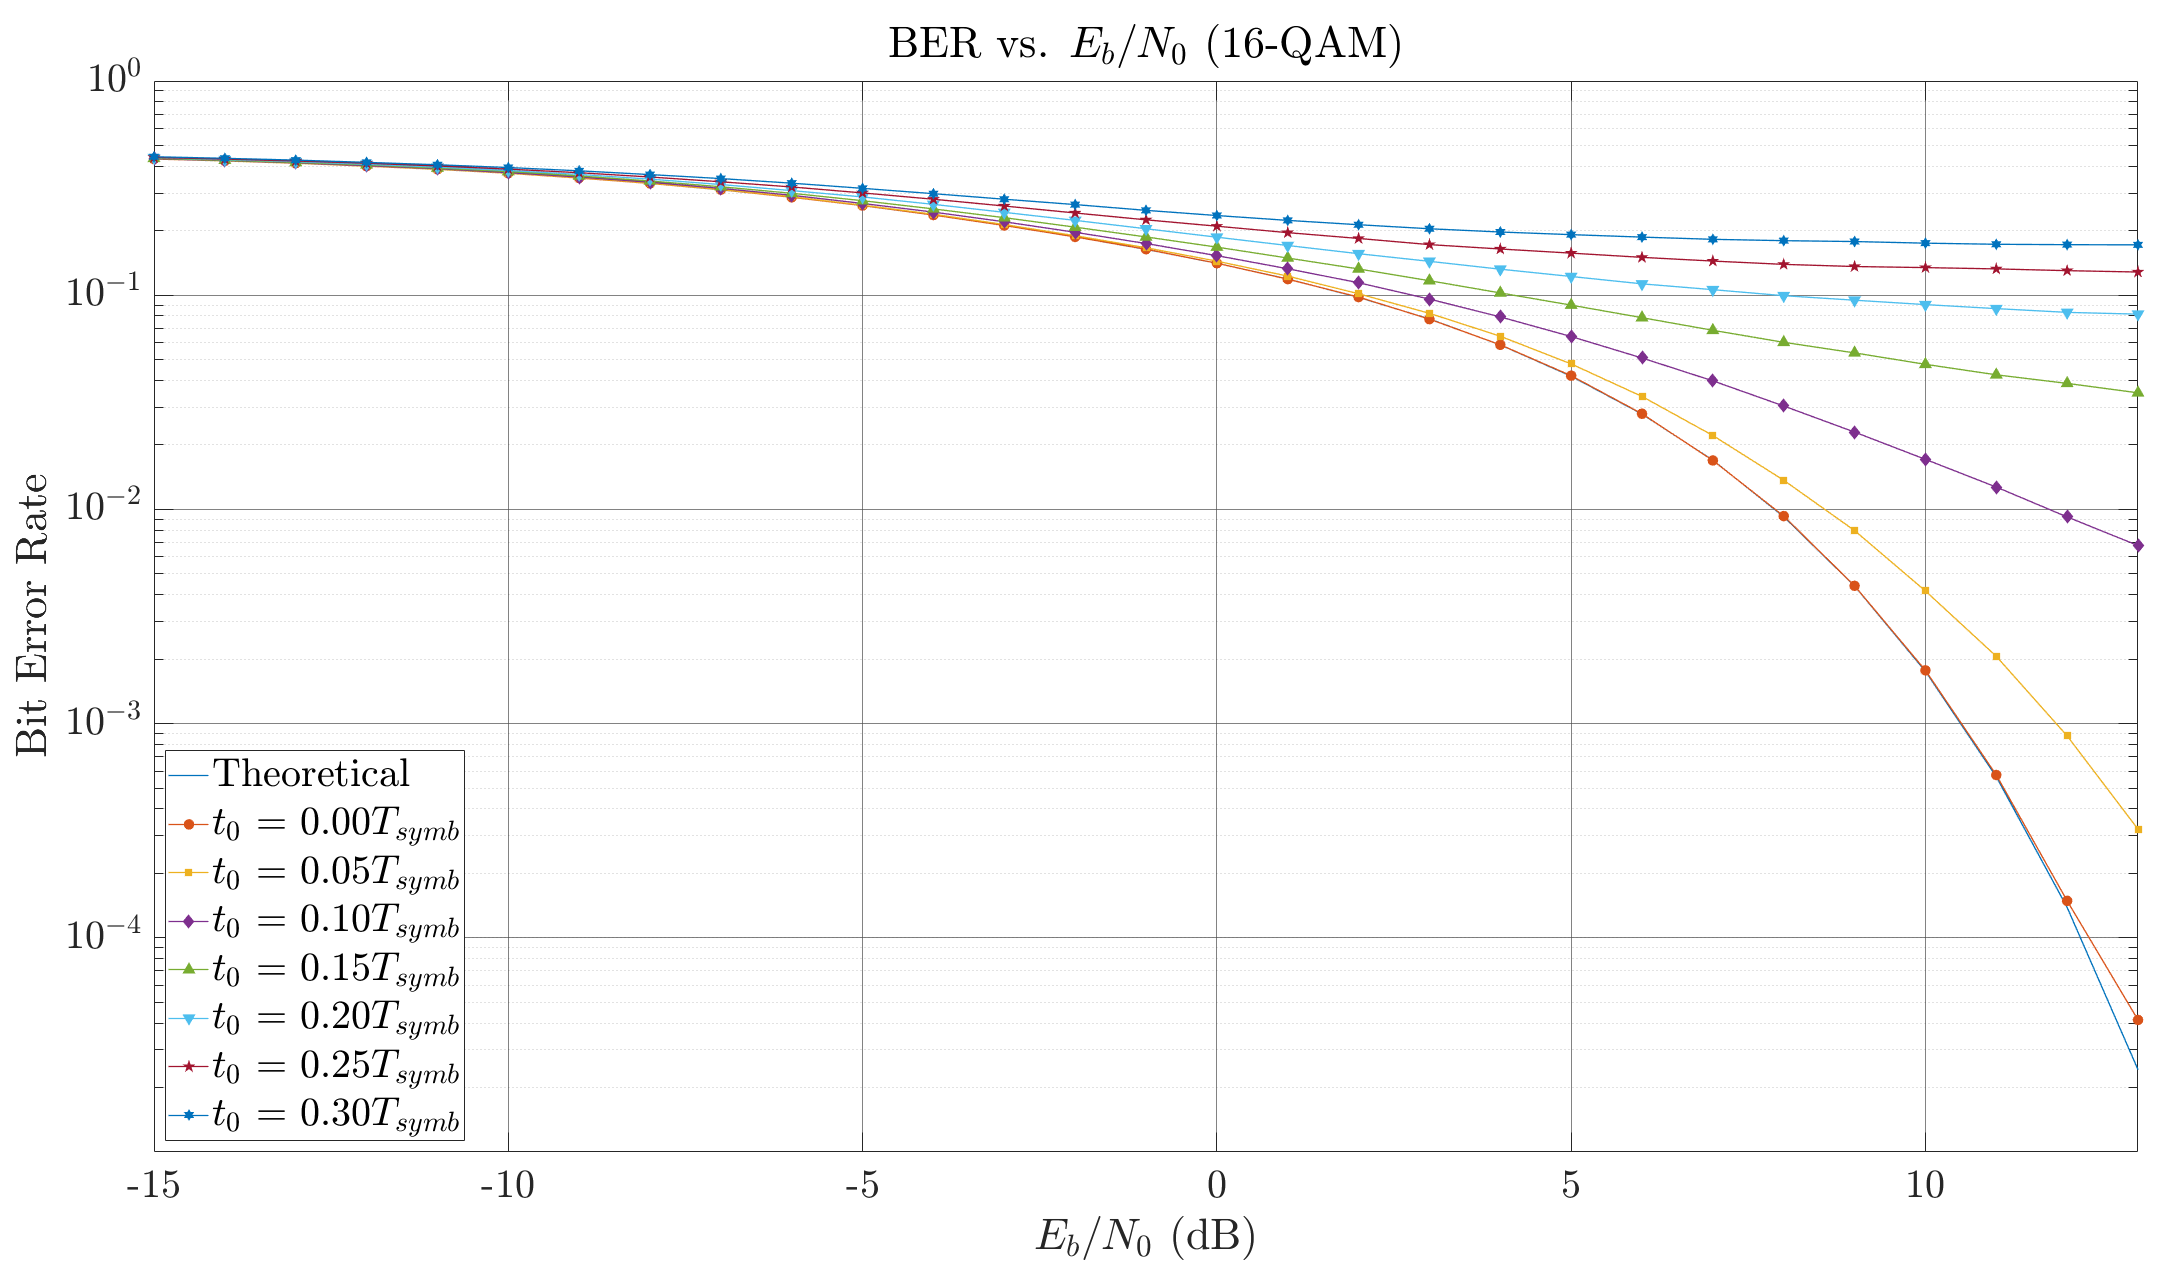
\includegraphics[width=\linewidth]{Images/ber-timing}
					\caption{BER vs. $E_b/N_0$ for varying $t_0/T_{symb}$.}
					\label{fig:ber-timing_compact}
				\end{subfigure}
				\caption{Impact of CFO and timing errors on BER for 16-QAM.}
				\label{fig:ber_sync_errors}
			\end{figure}
			
			\begin{figure}[H]
				\centering
				\begin{subfigure}[b]{0.48\textwidth}
					\centering
					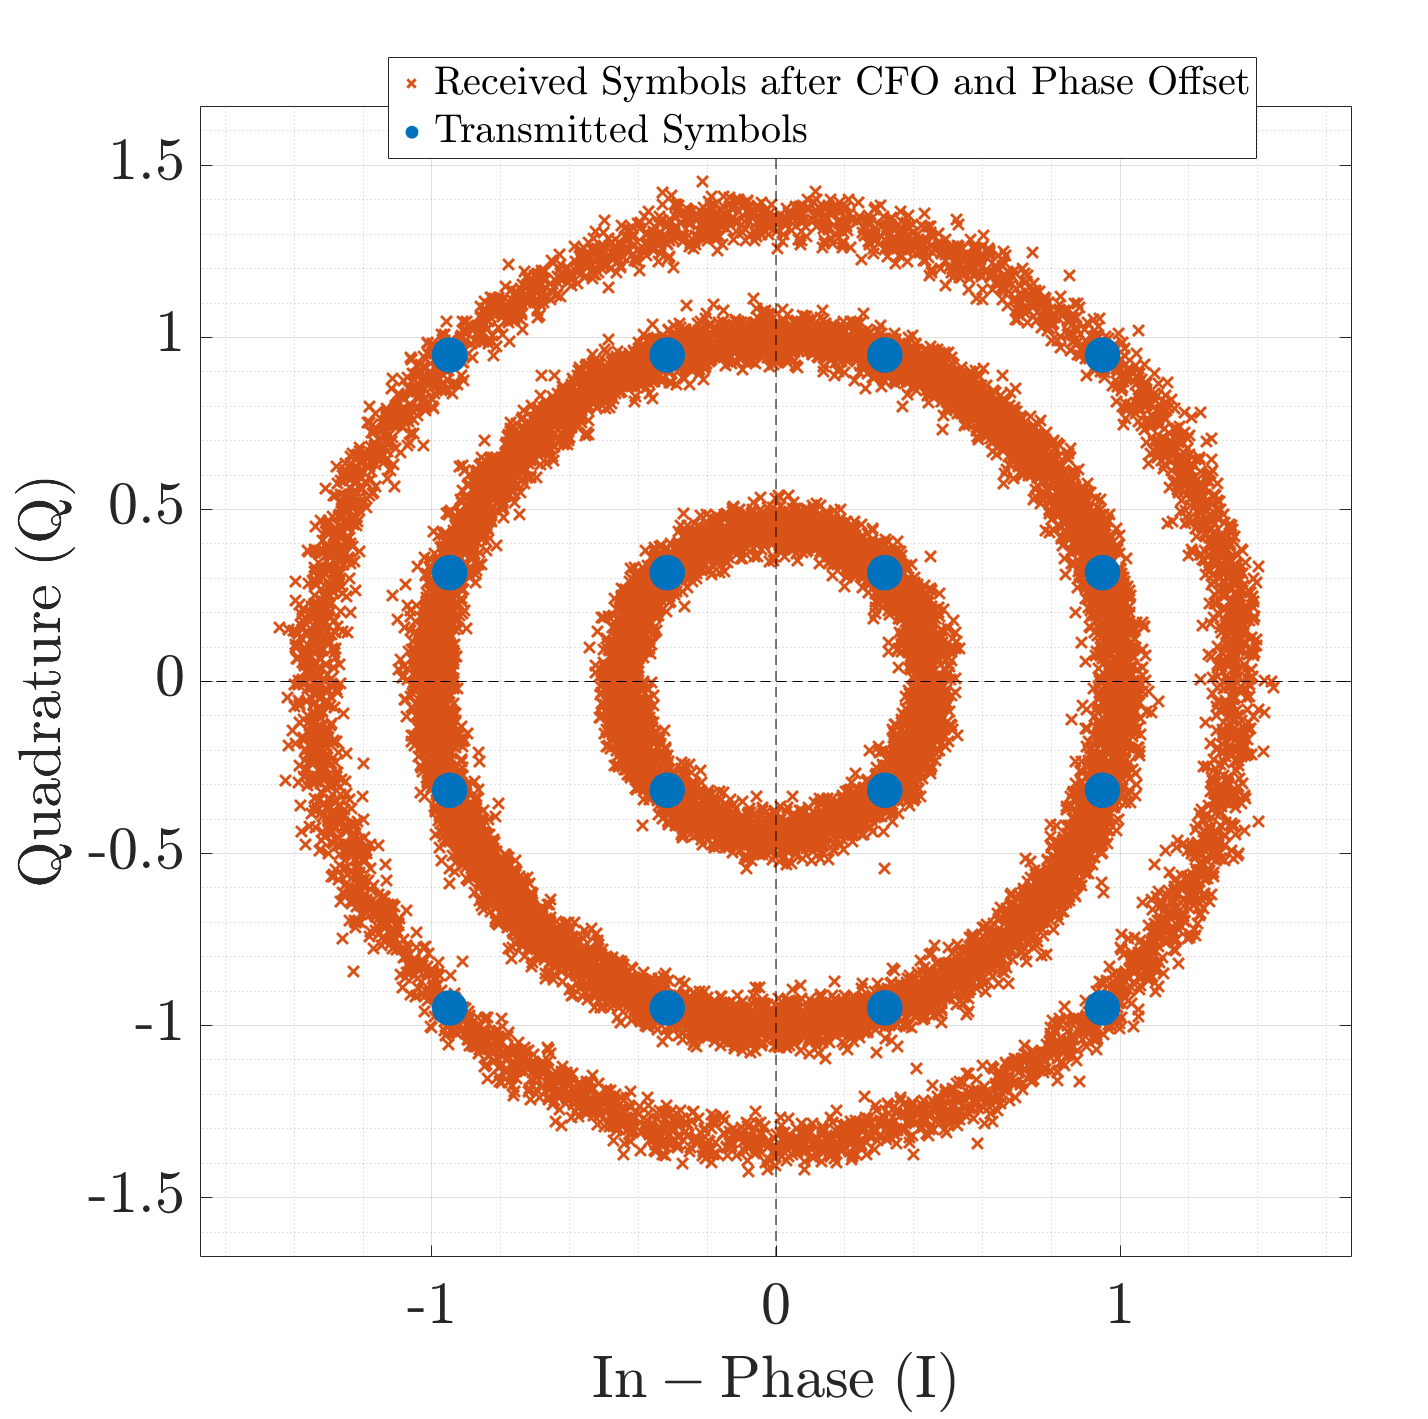
\includegraphics[width=\linewidth]{Images/cfo-po}
					\caption{Constellation with CFO and Phase Offset.}
					\label{fig:cfo-po-sub_compact}
				\end{subfigure}
				\hfill  
				\begin{subfigure}[b]{0.48\textwidth}
					\centering
					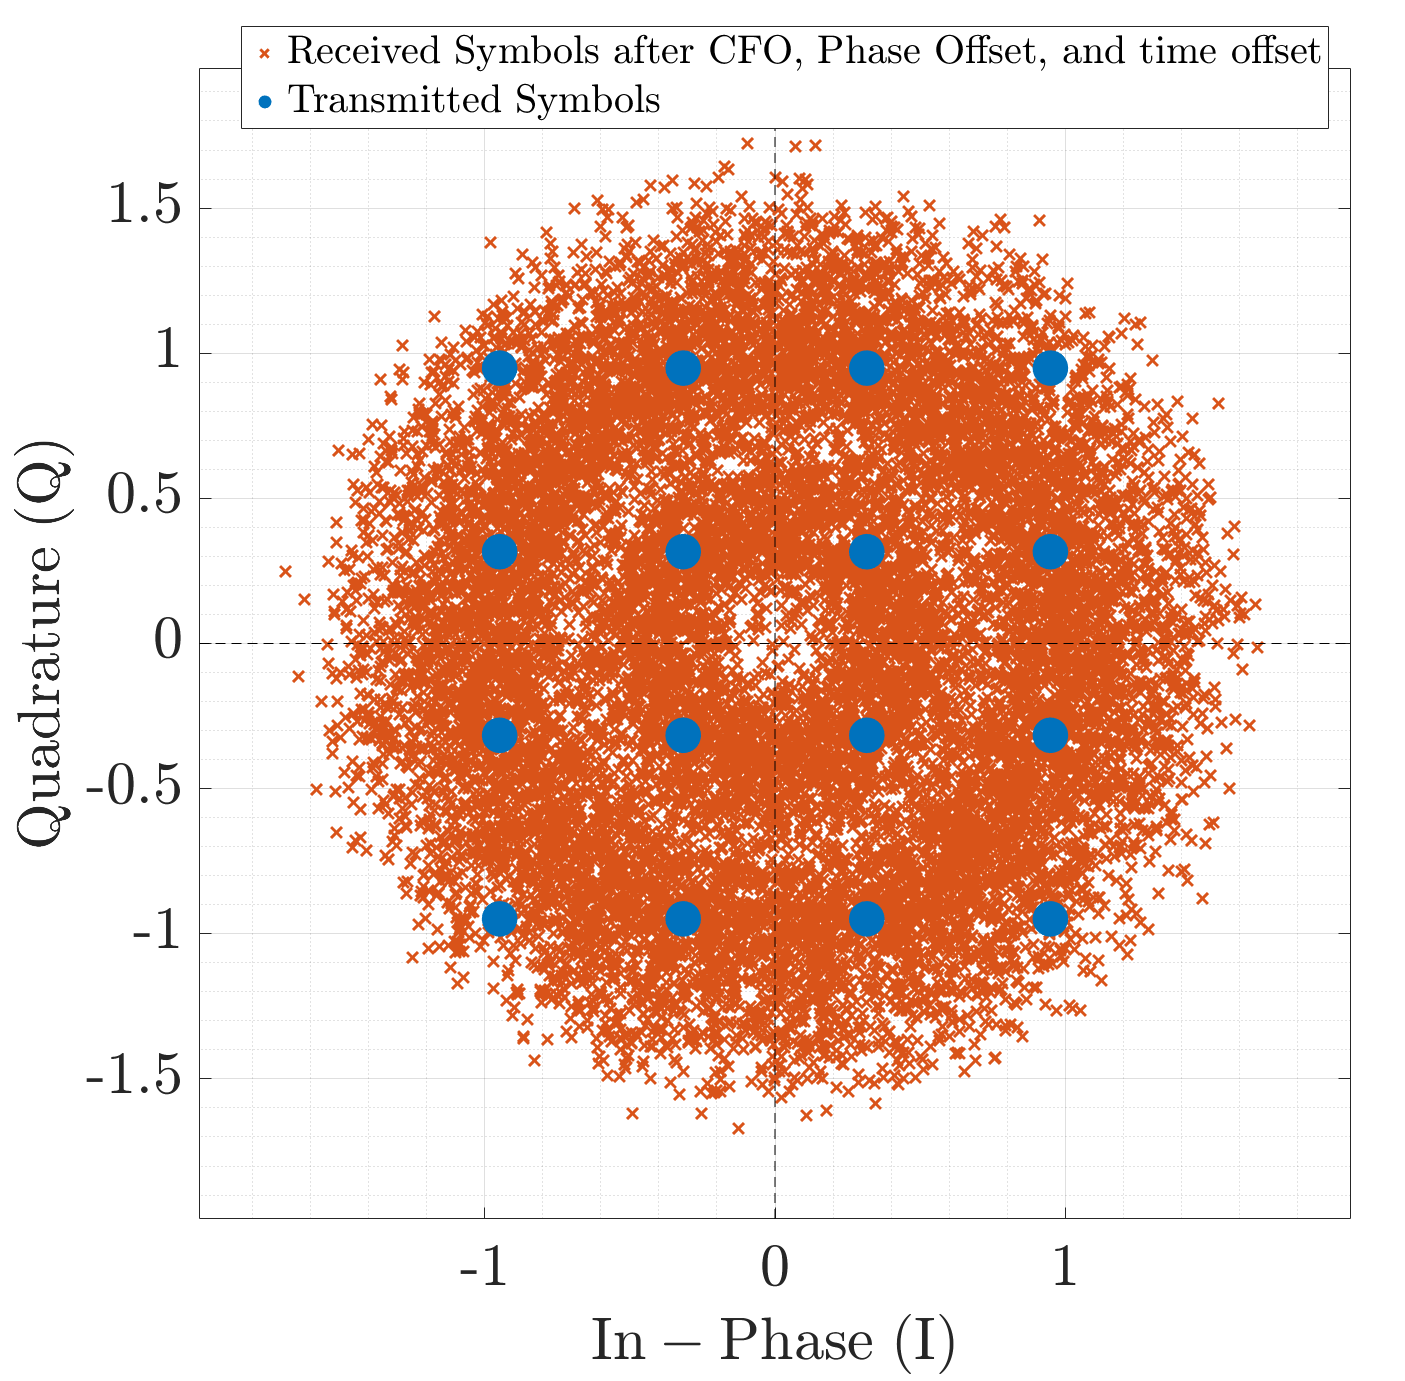
\includegraphics[width=\linewidth]{Images/cfo-po-to}
					\caption{Constellation with CFO, Phase Offset, and Time Offset.}
					\label{fig:cfo-po-to-sub_compact}
				\end{subfigure}
				\caption{Impact of synchronization errors on 16-QAM constellation ($E_b/N_0 = 20$ dB).}
				\label{fig:const_sync_errors}
			\end{figure}
			
			The Gardner algorithm, an NDA feedback loop, corrects sampling time errors $\epsilon[n]$. The update is:
			\begin{equation}
				\hat{\epsilon}[n+1] = \hat{\epsilon}[n] - \kappa \cdot \text{Re} \left\{ y_{\hat{\epsilon}[n]}[n-1/2] \left( y_{\hat{\epsilon}[n]}^{*}[n] - y_{\hat{\epsilon}[n-1]}^{*}[n-1] \right) \right\}
			\end{equation}
			Figure \ref{fig:gardner_performance} (a) shows convergence for different loop gains $\kappa$, and (b) demonstrates robustness to CFO.
			
			\begin{figure}[H]
				\centering
				\begin{subfigure}[b]{0.48\textwidth}
					\centering
					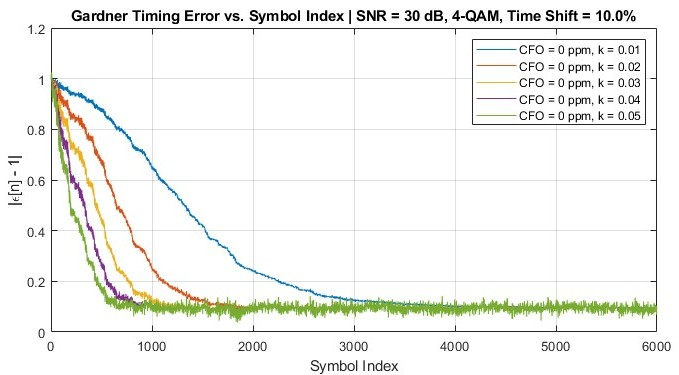
\includegraphics[width=\linewidth]{Images/Gardner_k_list.jpg} 
					\caption{Convergence for different $\kappa$.}
					\label{fig:gardner1_compact}
				\end{subfigure}
				\hfill
				\begin{subfigure}[b]{0.48\textwidth}
					\centering
					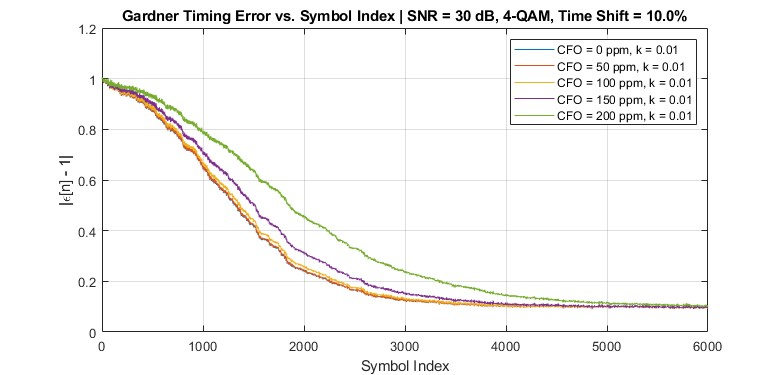
\includegraphics[width=\linewidth]{Images/Gardner_CFO_robust.jpg} 
					\caption{Robustness to CFO.}
					\label{fig:gardner2_compact}
				\end{subfigure}
				\caption{Gardner algorithm performance: time error convergence.}
				\label{fig:gardner_performance}
			\end{figure}
			
			Frame and coarse CFO acquisition use a DA differential cross-correlator with metric $D_k[n]$ from pilot $a[l]$:
			\begin{equation}
				D_k[n] = \frac{1}{N_p-k} \sum_{l=k}^{N_p-1} (y^*[n+l]a[l])(y^*[n+l-k]a[l-k])^*
			\end{equation}
			Pilot start $\hat{n} = \text{arg max}_n \sum_{k=1}^{K_{avg}} |D_k[n]|$. CFO $\hat{\Delta f} = -\frac{1}{K_{avg}} \sum_{k=1}^{K_{avg}} \frac{\angle D_k[\hat{n}]}{2\pi k T_{symb}}$. Figures \ref{fig:acquisition_vs_pilot_len_compact} and \ref{fig:acquisition_vs_K_avg_compact} show ToA and CFO estimation error standard deviations versus $E_b/N_0$ for varying pilot lengths $N_p$ and averaging windows $K_{avg}$, respectively. Longer pilots and optimized $K_{avg}$ improve accuracy.
			
			\begin{figure}[H]
				\centering
				\begin{subfigure}[b]{0.48\textwidth}
					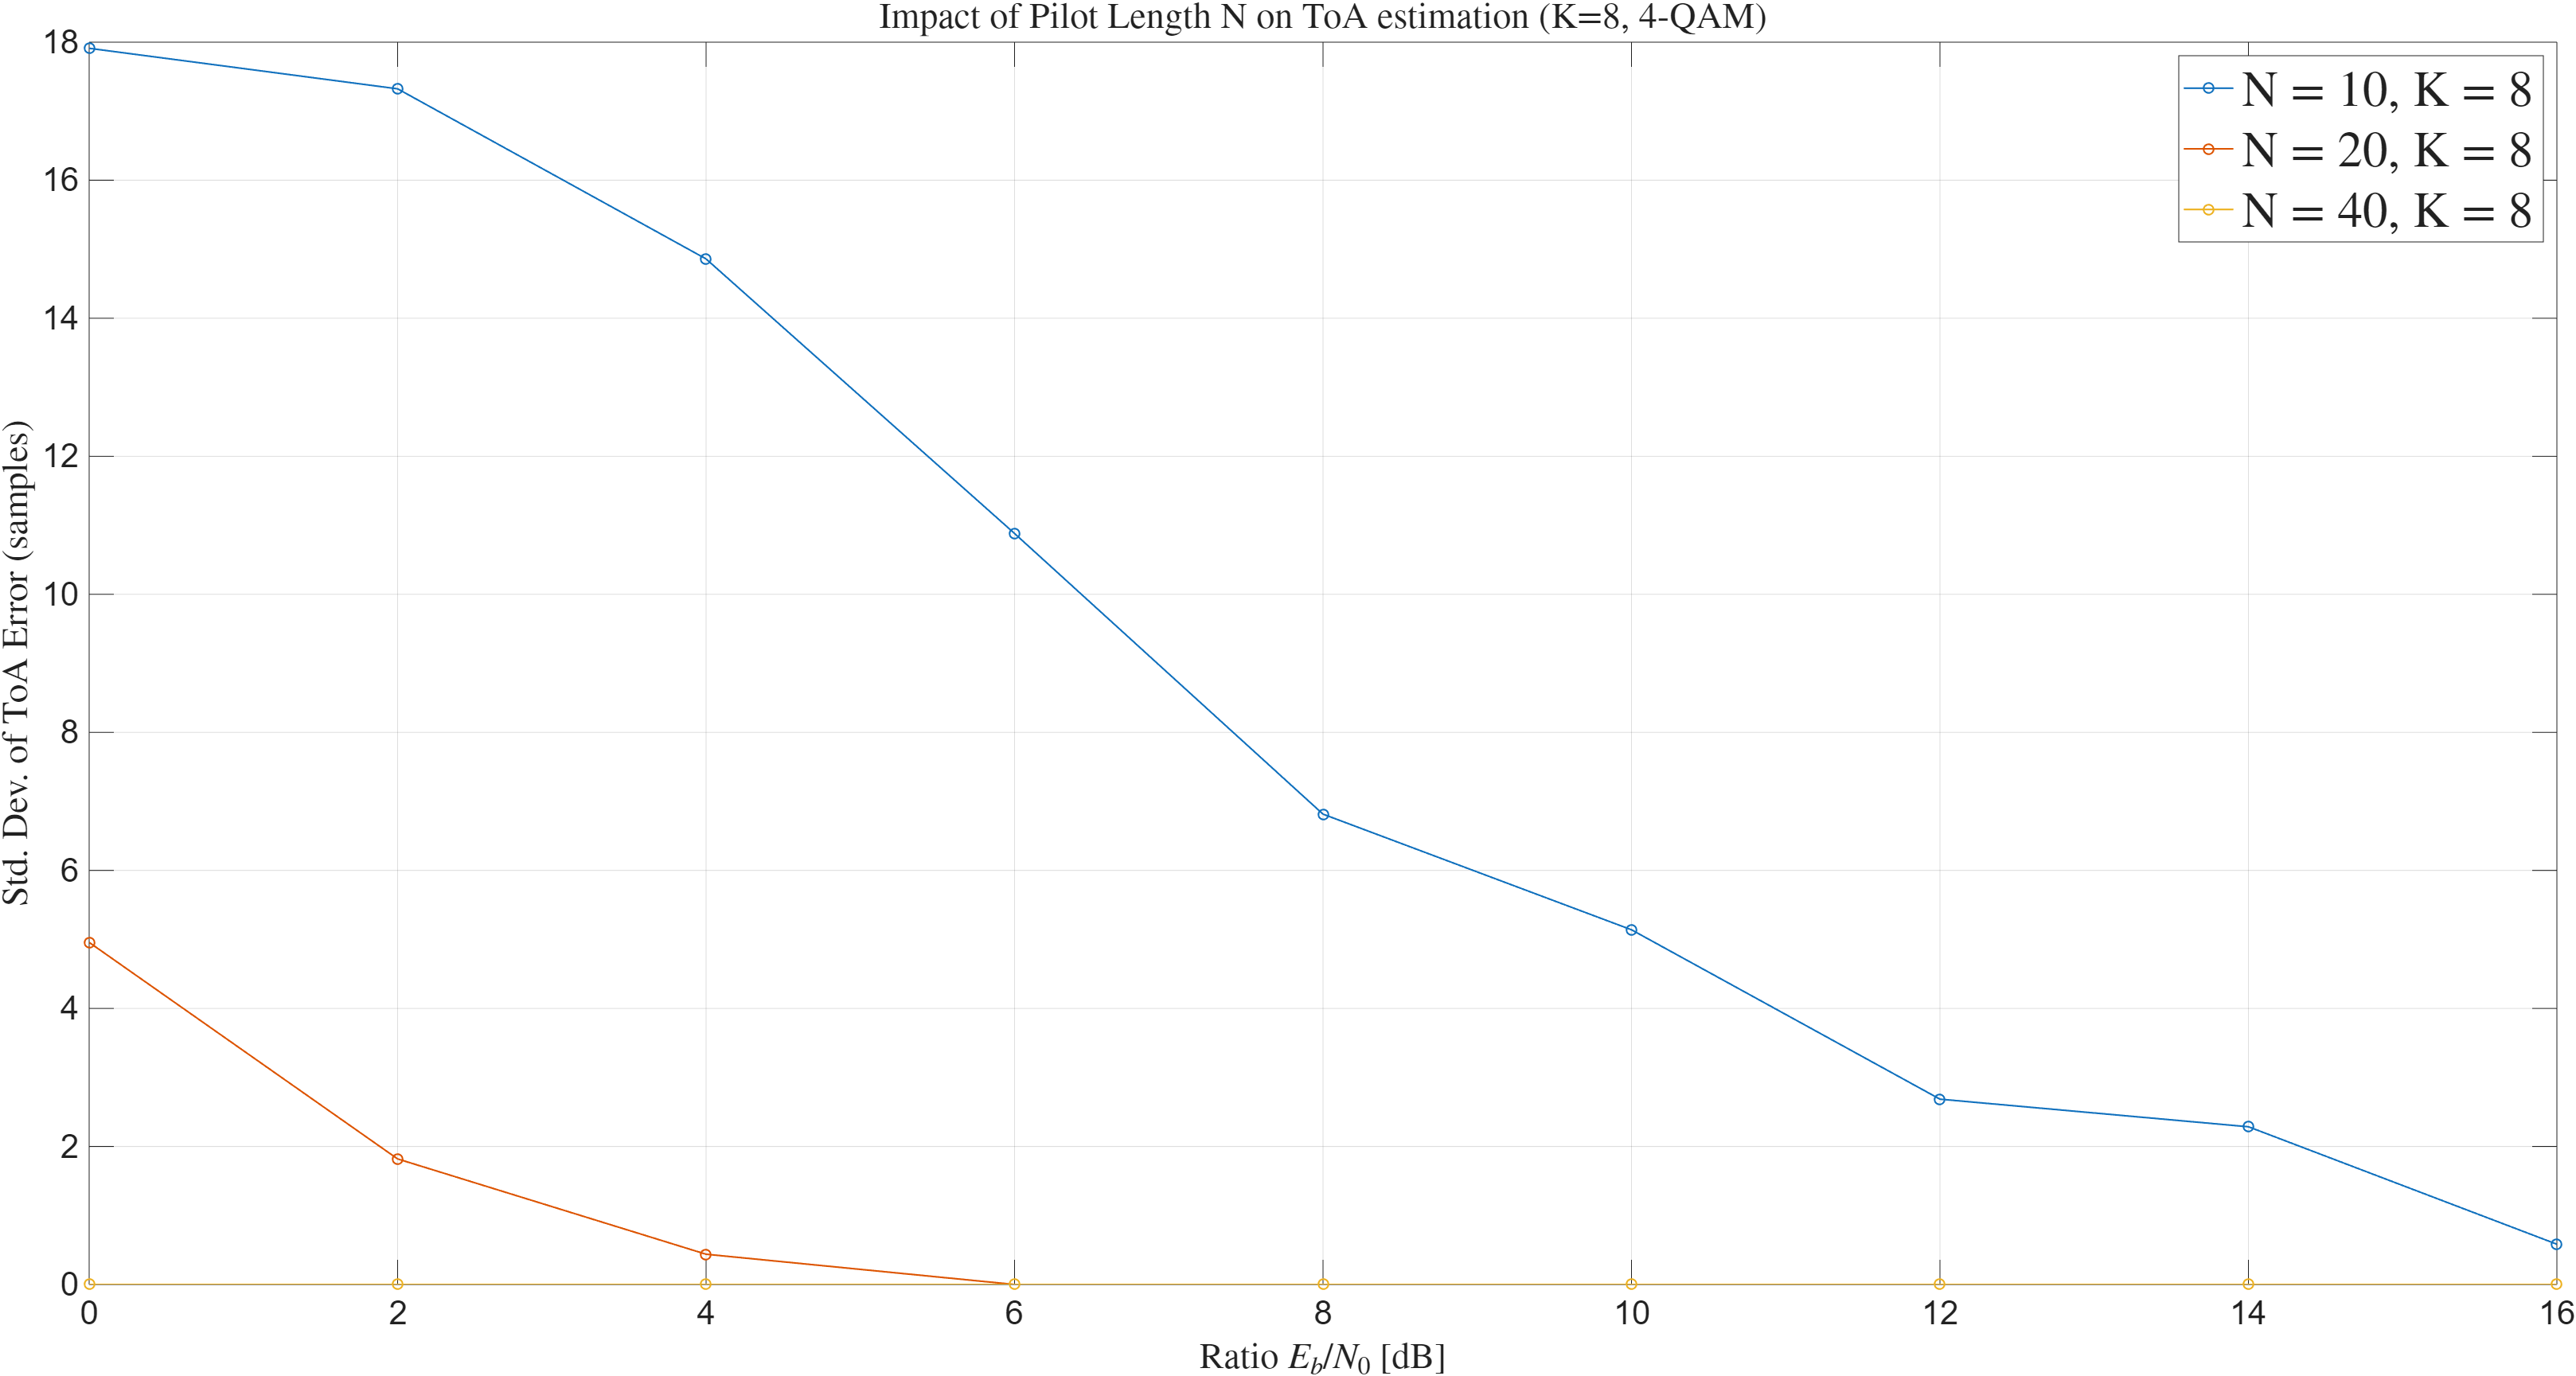
\includegraphics[width=\linewidth]{Images/frame_sync_pilot_len.png} 
					\caption{ToA error std dev vs. $N_p$.}
				\end{subfigure}
				\hfill
				\begin{subfigure}[b]{0.48\textwidth}
					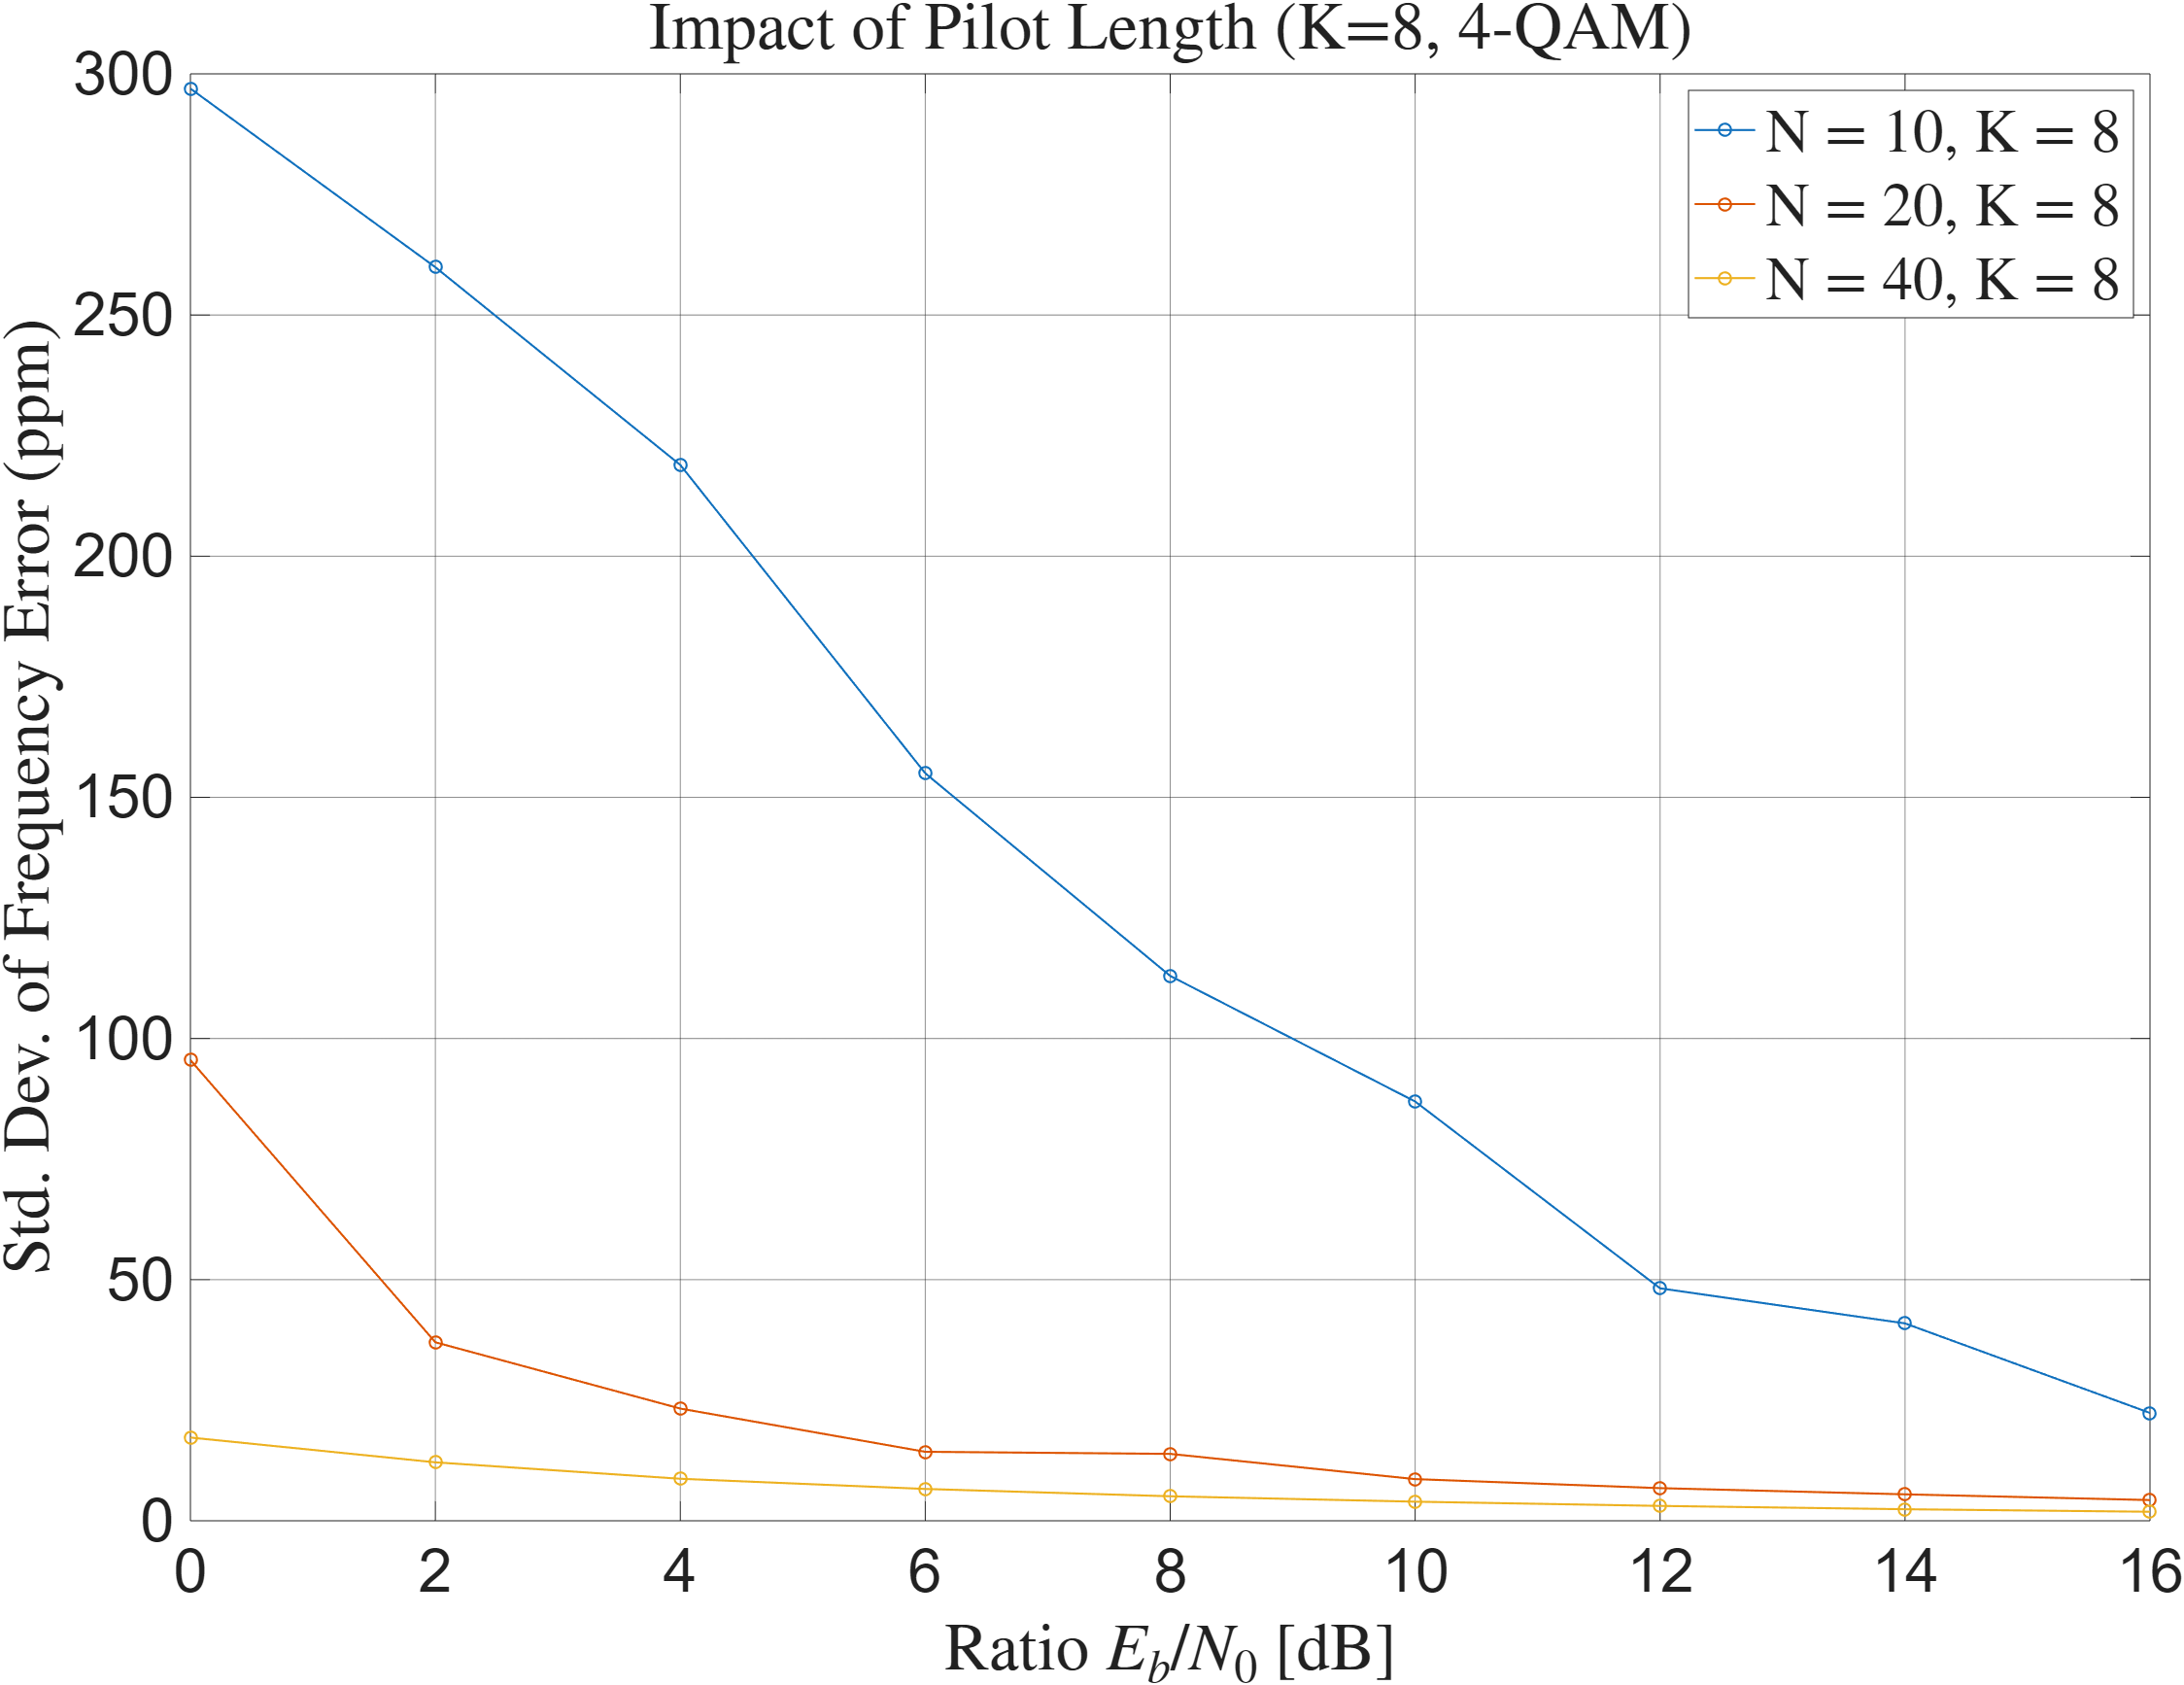
\includegraphics[width=\linewidth]{Images/cfo_est_pilot_len.png} 
					\caption{CFO error std dev vs. $N_p$.}
				\end{subfigure}
				\caption{Acquisition error vs. $E_b/N_0$ for different pilot lengths ($N_p$).}
				\label{fig:acquisition_vs_pilot_len_compact}
			\end{figure}
			
			\begin{figure}[H]
				\centering
				\begin{subfigure}[b]{0.48\textwidth}
					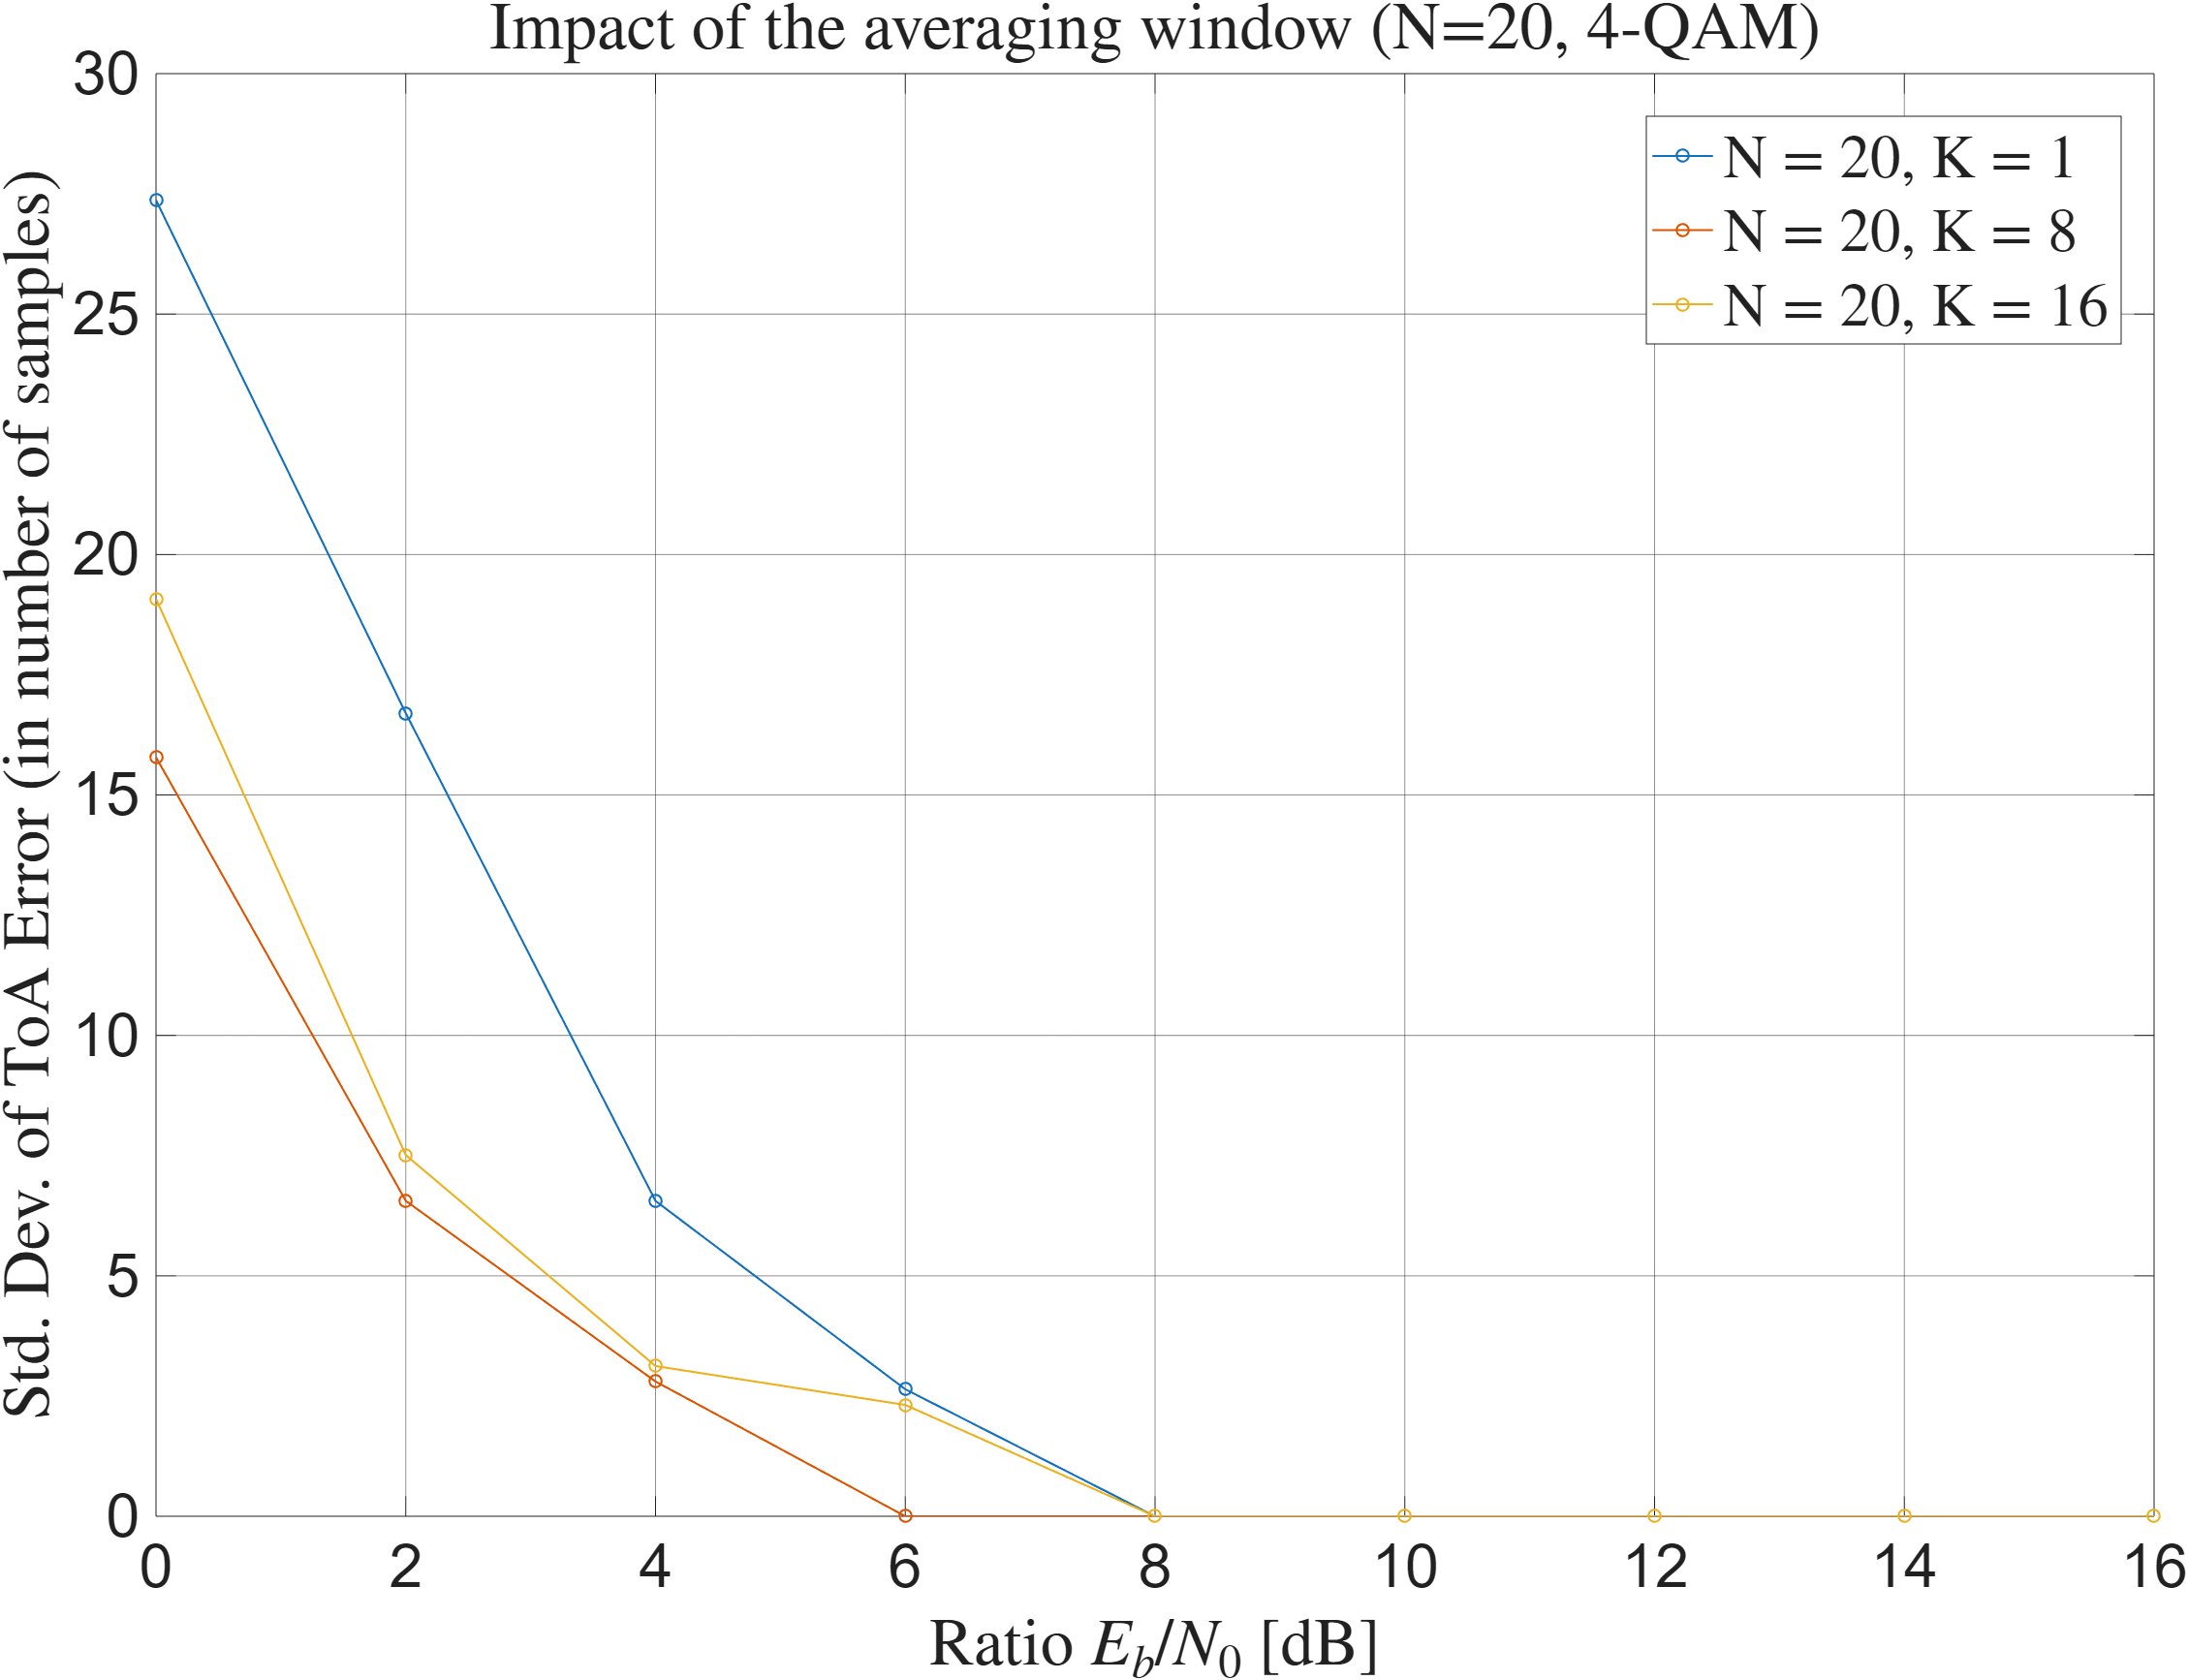
\includegraphics[width=\linewidth]{Images/frame_sync_K_avg.png} 
					\caption{ToA error std dev vs. $K_{avg}$.}
				\end{subfigure}
				\hfill
				\begin{subfigure}[b]{0.48\textwidth}
					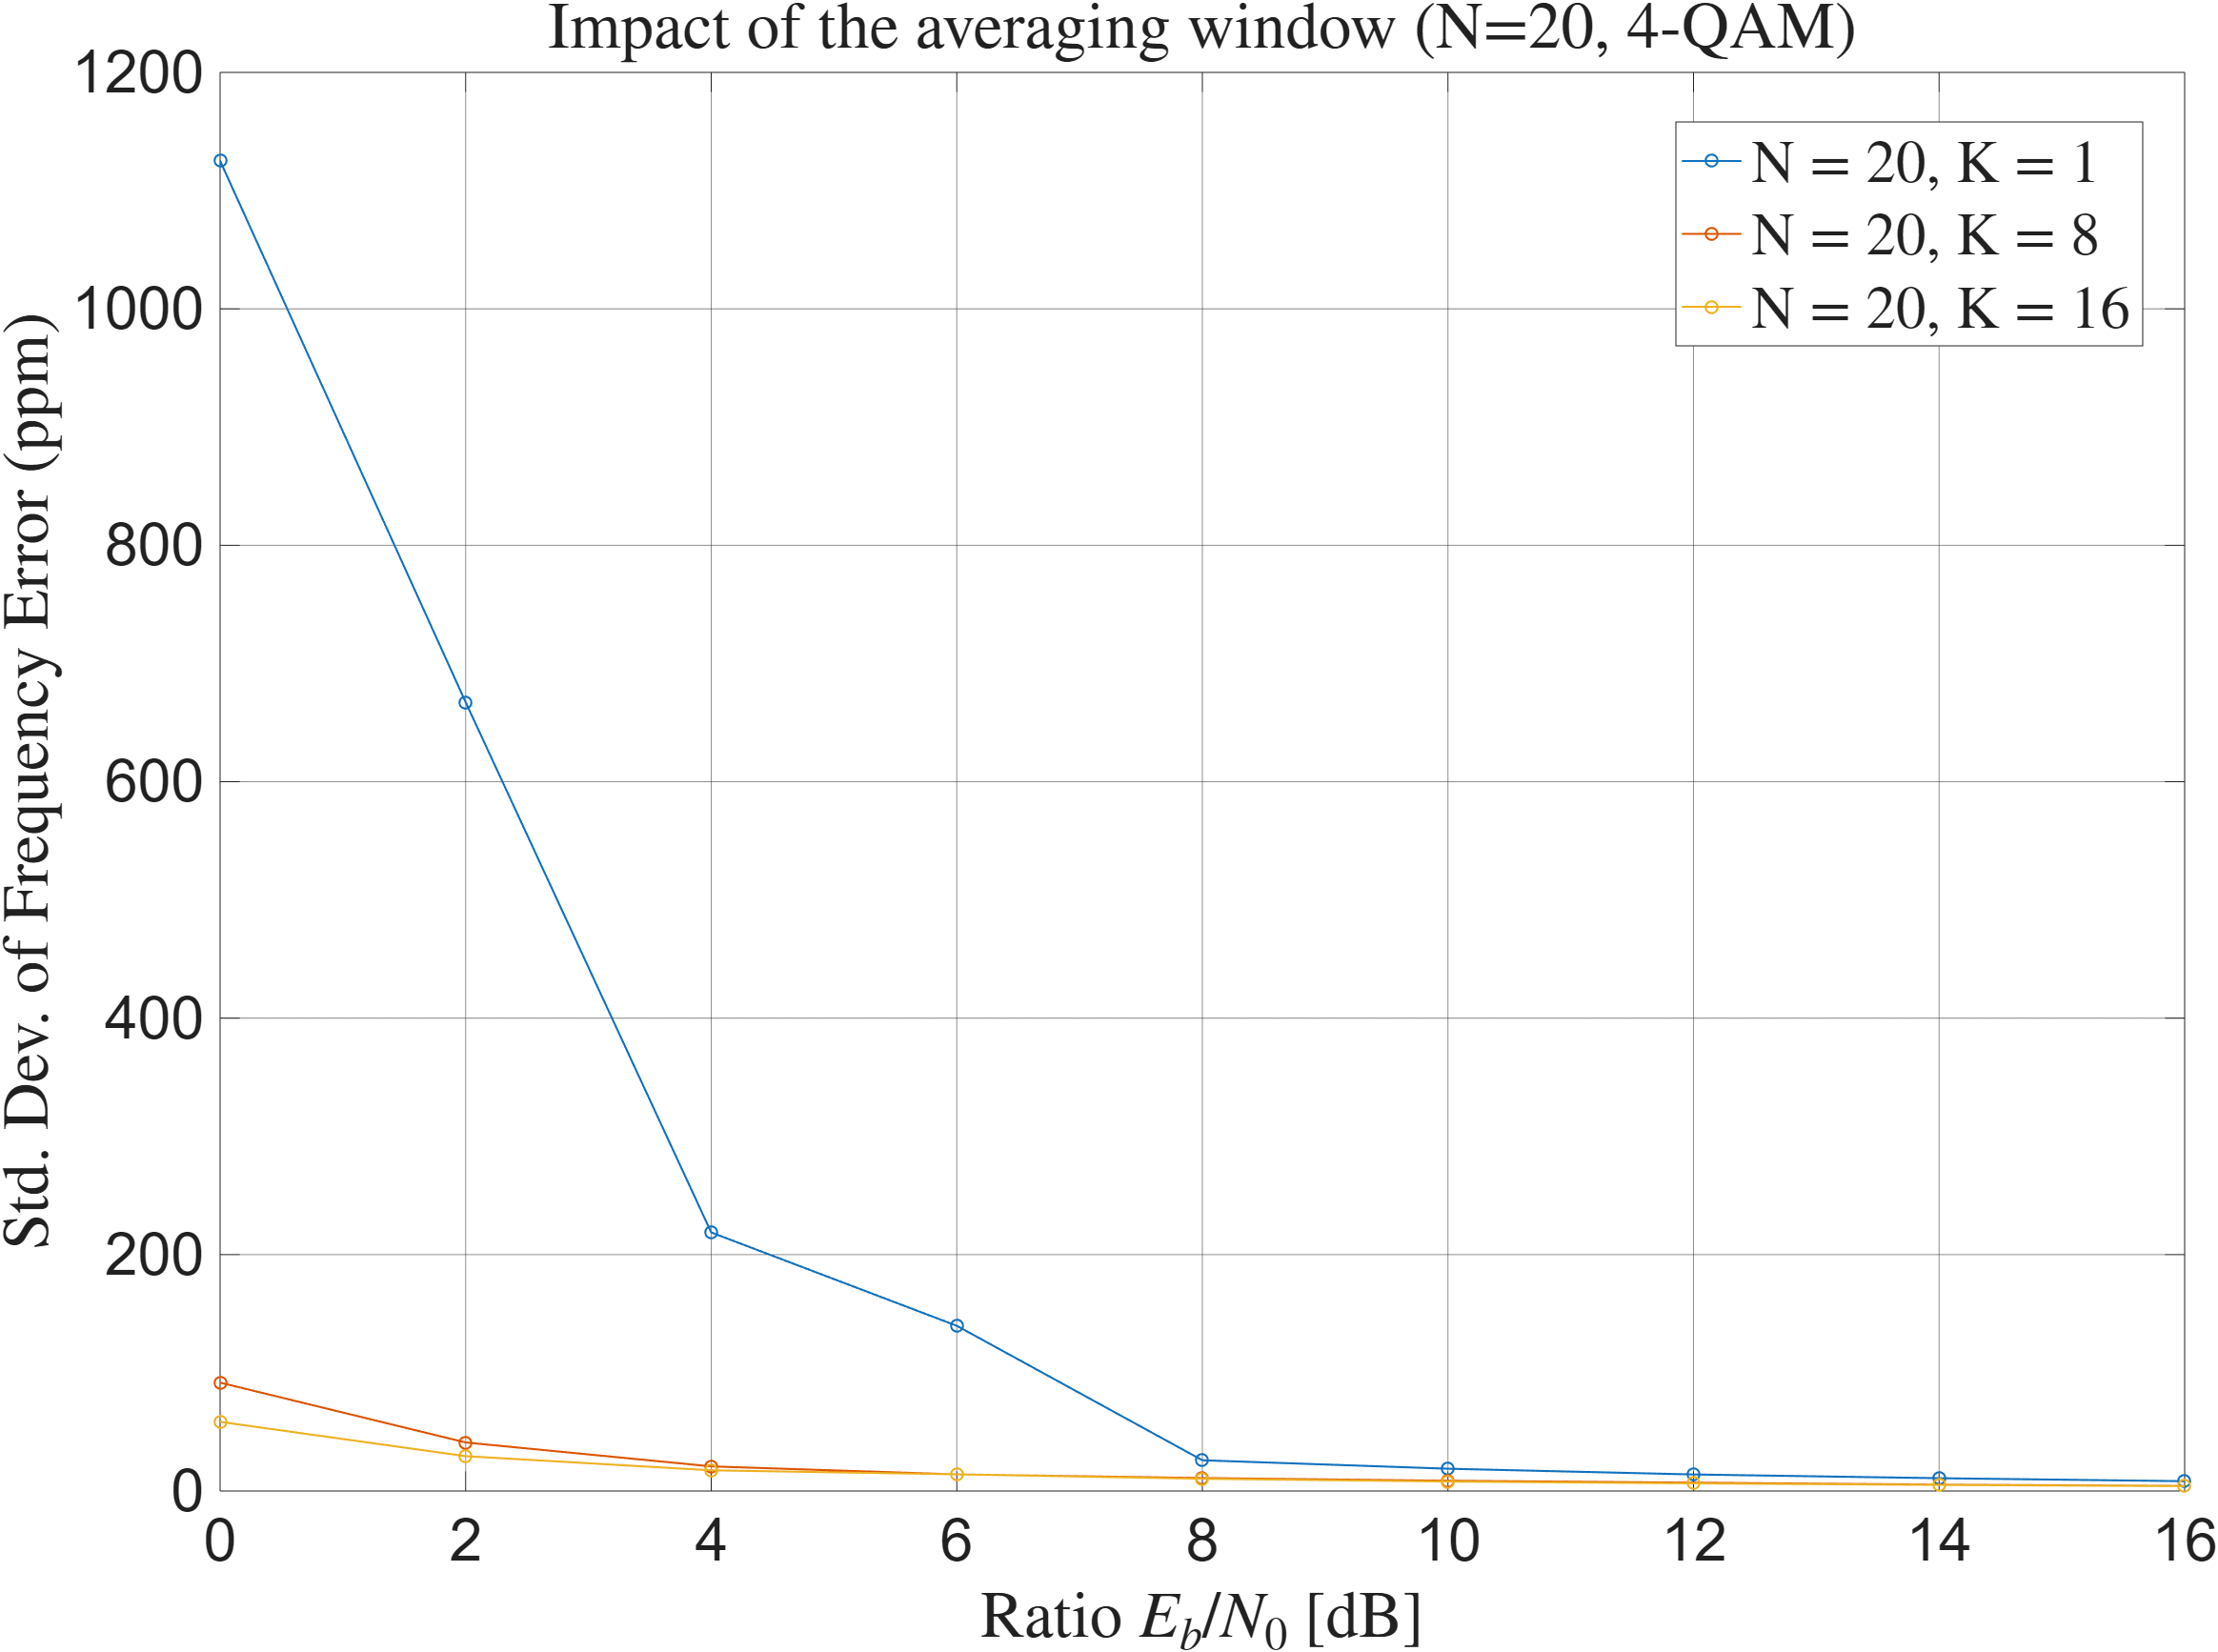
\includegraphics[width=\linewidth]{Images/cfo_est_K_avg.png} 
					\caption{CFO error std dev vs. $K_{avg}$.}
				\end{subfigure}
				\caption{Acquisition error vs. $E_b/N_0$ for different averaging windows ($K_{avg}$).}
				\label{fig:acquisition_vs_K_avg_compact}
			\end{figure}
			
			Residual phase error $\theta[n] = 2\pi \Delta f_{res} n T_{symb} + \phi_{res}$ after coarse CFO correction is handled by phase interpolation between pilot sequences. For a symbol at time $t$ between pilots at $t_1 (\hat{\theta}_1)$ and $t_2 (\hat{\theta}_2)$, correction $\hat{\theta}(t) = \hat{\theta}_1 + (\hat{\theta}_2 - \hat{\theta}_1) \frac{t - t_1}{t_2 - t_1}$. Figure \ref{fig:phase_interp_constellation_style_change_compact} demonstrates this correction.
			
			\begin{figure}[H]
				\centering
				\includegraphics[width=0.6\linewidth]{Images/phase_interp_constellation.png} 
				\caption{QAM constellation: before (smeared) and after (tightened) phase interpolation.}
				\label{fig:phase_interp_constellation_style_change_compact}
			\end{figure}
			
			The synchronization pipeline is: 1) Timing Recovery (Gardner), 2) Frame Acquisition, 3) Coarse CFO Acquisition, 4) Phase Interpolation. This order ensures robustness. Figure \ref{fig:const-corrected_compact} (repeated in \ref{fig:sync_overview_and_result} for overview) visually confirms the significant improvement in constellation clarity after Gardner and Frame/CFO acquisition, crucial for reliable demodulation.
			
			\subsection*{Questions: Time and Frequency Synchronization}
			\begin{projectquestion}{Baseband Model with Synchronization Errors:}
				Received baseband signal $\tilde{r}_e(t) = \tilde{s}(t-\epsilon T_{symb} - t_0) e^{j(2\pi\Delta f t + \phi_0)}$, where $\tilde{s}(t)$ is ideal transmitted baseband signal, $\epsilon$ is normalized clock offset, $t_0$ time shift, $\Delta f$ CFO, $\phi_0$ phase offset. For sampling at $nT_{symb}(1+\delta)+t_0'$, considering $y[n]$ as output of matched filter and ADC.
			\end{projectquestion}
			
			\begin{projectquestion}{Separating Phase Drift and ISI from CFO:}
				Phase drift from CFO is $e^{j2\pi \Delta f nT_{symb}}$ on symbols $I[n]$. ISI results from $g(t)e^{j2\pi\Delta ft}$ convolved with $g^*(-t)$ not being a perfect Nyquist pulse. To see ISI alone, multiply received symbols by $e^{-j2\pi \Delta f nT_{symb}}$ after matched filtering to remove coherent phase rotation, then observe BER degradation.
			\end{projectquestion}
			
			\begin{projectquestion}{Simulating Sampling Time Shift:}
				Increase sampling rate by large factor $M_{os}$ pre-filter. A shift of $k$ samples at this high rate corresponds to $t_0 = k \cdot T_{symb}/M_{os}$. Alternatively, use interpolation on the oversampled signal at the receiver output to estimate values at $nT_{symb} + t_0$.
			\end{projectquestion}
			
			\begin{projectquestion}{Selecting $E_b/N_0$ for Synchronization Tests:}
				$E_b/N_0$ must be high enough for synchronization algorithms to lock and provide meaningful performance metrics without being dominated by noise failures. Typically, choose values where uncoded BER is reasonably low (e.g., $10^{-2}$ to $10^{-4}$), or a typical operating point. For some algorithms, a minimum $E_b/N_0$ (e.g., > 4-6 dB) is needed for reliable acquisition, as seen in frame/frequency acquisition plots.
			\end{projectquestion}
			
			\begin{projectquestion}{Selecting Pilot and Data Sequence Lengths:}
				Pilots ($N_p$): Long enough for accurate ToA/CFO/Phase estimation against noise (e.g., $N_p \ge 20-40$). Too short leads to high estimation variance.
				Data: Short enough between pilots to ensure phase drift from residual CFO is < $\pi$ (for unambiguous phase interpolation) and linear phase change assumption holds.
				Trade-off: Longer/more frequent pilots improve sync but reduce data throughput (overhead).
			\end{projectquestion}
			
			\begin{projectquestion}{Order of Synchronization Operations:}
				1. Timing Recovery (Gardner): Robust to CFO.
				2. Frame/Frequency Acquisition (Differential Cross-correlator): Uses timed samples to find frame start and correct large CFO.
				3. Phase Tracking/Interpolation: Corrects residual phase errors.
				This order allows each stage to operate on a signal pre-processed to mitigate errors that would impair its own performance.
			\end{projectquestion}
			
			\begin{projectquestion}{Gardner Algorithm Error Computation and CFO Robustness:}
				Error: $e[n] = \text{Re} \{ y[n-1/2] ( y^{*}[n] - y^{*}[n-1] ) \}$. $y[n-1/2]$ is the mid-point sample. $(y^{*}[n] - y^{*}[n-1])$ estimates signal slope. If $y[n-1/2]$ and slope have same sign, timing is late; opposite sign, early. No transition means small slope, small update.
				Robustness to CFO: CFO causes phase rotation $\Delta\phi = 2\pi \Delta f T_{symb}$ between $y[n-1]$ and $y[n]$, and $\Delta\phi/2$ on $y[n-1/2]$. The error term uses $\text{Re}\{\cdot\}$. For small $\Delta\phi$ per symbol (typical CFOs), $e^{j\Delta\phi} \approx 1+j\Delta\phi$. The dominant terms in the error calculation are less affected by these small phase rotations.
			\end{projectquestion}
			
			\begin{projectquestion}{Differential Cross-Correlator vs. Usual Cross-Correlator:}
				Usual cross-correlator ($C[n] = \sum y^*[n+l]a[l]$) is sensitive to CFO, as CFO rotates $y[n+l]$ causing phase terms $e^{j2\pi\Delta f (n+l)T_{symb}}$ that don't cancel in $|C[n]|$, degrading the peak.
				Differential cross-correlator (Eq. \ref{eq:diff_corr_metric_style_change}) multiplies two correlation terms with a time lag $k$. The product $(y^*[n+l]a[l])(y[n+l-k]a^*[l-k])$ has phase $e^{-j2\pi\Delta f(n+l)T_{symb}} \cdot e^{j2\pi\Delta f(n+l-k)T_{symb}} = e^{-j2\pi\Delta f k T_{symb}}$. The phase is proportional to $k\Delta f$, allowing $\Delta f$ estimation. The magnitude is less affected by the absolute phase.
				Summation for $k=0$: $D_0[n] = \frac{1}{N_p}\sum |y[n+l]a[l]|^2$, which relates to energy detection but doesn't directly use the differential property for CFO estimation. The CFO estimation relies on $k \ge 1$.
			\end{projectquestion}
			
			\begin{projectquestion}{Optimality of Frame/Frequency Acquisition Algorithms:}
				The ML criterion for joint ToA ($\hat{n}$) and CFO ($\Delta\omega$) estimation is $(\hat{n},\Delta\omega)= \text{arg max}_{n,\omega} p(y[n]|a,\Delta\omega)$. Direct implementation is complex (2D search over $n$ and $\omega$). The differential cross-correlator is a near-optimal, lower-complexity approximation. It's not strictly ML optimal because it simplifies the likelihood function or uses derived metrics, often omitting terms like received signal power that an exact ML estimator might include.
			\end{projectquestion}
			
		\end{document}